% !TeX spellcheck = en_GB
\documentclass[a4paper, 12pt]{book}
\usepackage[utf8]{inputenc}
\usepackage[english]{babel}
\usepackage{amsmath}
\usepackage{amsfonts}
\usepackage{amssymb}
\usepackage{amsthm}
\usepackage{array}
\usepackage{mathtools}
\usepackage{graphicx}
\usepackage{hyperref}
\usepackage{caption}
\usepackage{cancel}
\usepackage{subcaption}
\usepackage{comment}
\usepackage{geometry}
\usepackage{lipsum}


%\usetikzlibrary{decorations.text}

\newtheorem{theorem}{Theorem}[chapter]
\newtheorem{proposition}[theorem]{Proposition}
\newtheorem{defin}[theorem]{Definition}
\newtheorem{cor}[theorem]{Corollary}
\newtheorem{lemma}[theorem]{Lemma}
\newtheorem{oss}[theorem]{Remark}
%
%\newtheorem{theor}{Teorema}[chapter]
%\newtheorem{lemma}[theor]{Lemma}
%\newtheorem{prop}[theor]{Proposizione}
%\newtheorem{coroll}[theor]{Corollario}

%
%\theoremstyle{definition}
%\newtheorem{defn}{Definizione}[chapter]
%\newtheorem{ex}{Esempio}[chapter]
%\newtheorem*{definizione-numr}{Definizione}
%
%\theoremstyle{remark}
%\newtheorem{oss}{Osservazione}[chapter]
%
%
%\newenvironment{skproof}{%
%	\renewcommand{\proofname}{Sketch di dimostrazione}\proof}{\endproof}
%\newenvironment{necproof}{%
%\renewcommand{\proofname}{Dimostrazione della necessarietà}\proof}{\endproof}
%\newenvironment{sufproof}{%
%\renewcommand{\proofname}{Dimostrazione della sufficienza}\proof}{\endproof}
%
\newcommand{\R}{\mathbb{R}}
\newcommand{\ttl}{THE ALEXANDROV MOVING PLANE METHOD \\AND APPLICATIONS TO GEOMETRIC FLOWS}

\author{Marco Tamburro \\ Relatore: Carlo Sinestrari}
\title{\ttl}
\date{\today}

\newenvironment{localsize}[1]
{%
	\clearpage
	\let\orignewcommand\newcommand
	\let\newcommand\renewcommand
	\makeatletter
	\input{size#1.clo}%
	\makeatother
	\let\newcommand\orignewcommand
}
{%
	\clearpage
}

\begin{document}

%\maketitle 
%\frontmatter
\begin{localsize}{11}
	\thispagestyle{empty}
%\begin{figure}
%\centering
%
\includegraphics[scale=1.5]{logo.png}
%\end{figure}
\begin{center}
	University logo Placeholder\vspace{70pt}
\end{center}

\begin{center}
\textsc{Università degli studi di Roma "Tor Vergata" \\ Dipartimento di Matematica \\ Corso di laurea magistrale in Matematica}
\end{center}
\vspace{25pt}
\begin{center}
\textbf{\Large{TBC}}
\end{center}
\vspace{60pt}
\begin{flushleft}
Relatore: \\ Chiar.mo Prof. \textbf{Carlo Sinestrari}
\end{flushleft}
\vspace{70pt}
\begin{flushright}
Tesi di laurea di: \\ \textbf{Marco Tamburro}\\
\vspace{1pt}
Matricola: 0318523
\end{flushright}
\thispagestyle{empty}
\vspace{109pt}
\begin{center}
	Anno Accademico 2021-2022
\end{center}
\newpage
\end{localsize}
\tableofcontents

\phantomsection
% !TeX spellcheck = en_GB
\chapter*{Introduction}
\addcontentsline{toc}{chapter}{Introduction}

This Master's thesis analyses the Alexandrov Moving Planes Method and its applications to Geometric Flows. 

The main original result in this thesis is the extension of a result from Chow and Gulliver about flows in Euclidean space to  the case where the ambient space is constant curvature spaces. Moreover, in the last chapter, we include a new proof - using the moving planes method - of the well known result stating that some area-preserving and volume-preserving flows do not leave a large enough compact. 

The Moving Planes Method is a technique in Analysis that can be used to prove radial symmetry of certain solutions to some differential equations. To apply the method, one considers a solution and its reflections about a foliation of the ambient space by geodesic hyperplanes. The method consists of reflecting the part of a solution ``below" the hyperplane into the top part, and using properties of both copies of the solution together, generally some form of maximum principle, to prove some property of the non-reflected solutions. The method was originally used to analyse geometric elliptic PDEs, and it is now an important tool in Geometric Analysis

The central result is a theorem by Chow and Gulliver (theorem \ref{chow gulliver}) contained in a 1997 paper \cite{Chow}, who proved that the method \textit{behaves well} with respect to certain parabolic geometric flows. 


We consider manifolds $M^n$ embedded in $\R^{n+1}$, i.e. there is an embedding $X_0 : M^n \rightarrow \R^{n+1}$ parametrizing the hypersurface $X_0(M^n)$ evolving according to a geometric flow in the form: 

\begin{align*}
	\begin{dcases}
		\frac{\partial X_t}{\partial t} = - F(\kappa_1(x), \dots , \kappa_n(x)) \nu\\
		X(0)= X_0
	\end{dcases} 
\end{align*}
where $\nu$ is the outward normal to $X_t(M^n)$ at the point $X_t(x)$, $\kappa_1\leq \dots \leq \kappa_n$ are the principal curvatures at $X_t(x)$, and 
\begin{align*}
	\frac{\partial F}{\partial \kappa_i} > 0 \mathrm{\; for \; all } \; i=1,\dots, n
\end{align*}

The Chow-Gulliver result states:

\begin{theorem*}[Chow-Gulliver]
	Let $X:M^n\times [0,T) \rightarrow \R^{n+1}$ be a $C^2$ solution to equation the equation above. Then, if we can reflect $X(M^n, 0)=X_0$ strictly with respect to $\pi$, then for all $t\in [0,T)$ we can reflect $X(M^n, t)=X_t$ strictly with respect to $\pi$. 
\end{theorem*}

Here by strict reflection we mean that the following two conditions are met: 
\begin{itemize}
	\item The half of the manifold above the plane reflects inside the other half of the manifold, without touching it.
	\item The tangent spaces of the manifold and its reflection about the plane do not coincide at any point on the plane.
\end{itemize}

The key idea in the proof of the result is as follows: suppose we have an embedded smooth hypersurface $X$ evolving according to the equation above and a fixed hyperplane $\pi$, intersecting $X$. Suppose that, at some time $t$, $X$ and  its reflection about the hyperplane $X_\pi$ touch at a point not on $\pi$. We can consider $X$ and  $X_\pi$ as local graphs over the same hyperplane $\pi$, and we can show that these function evolve according to the same differential equation. Using the strong maximum principle and the Hopf boundary point lemma, then, one can conclude that the two functions coincide, and have been coinciding up until that point. In particular, if at some time $t$ a solution and its reflection do not touch, they will not touch for all subsequent times. 

In the first chapter, some foundational results are collected. Firstly, some equations in local coordinates for immersed hypersurfaces are derived and some well known theorems in differential geometry and on parabolic differential equations are stated, and proved when necessary. A version of the maximum principle and of Hopf's boundary point lemma for non-linear equations is introduced in section \ref{non linear pde parabolic section}.

After that, in section \ref{reflections definitions} and 
\ref{method moving planes} we introduce the notation for reflections in constant-curvature spaces and the Alexandrov Moving Planes Method. A sketch of the proof of the Alexandrov soap-bubble theorem is included in the last section of the chapter, to show an application of the technique to elliptic differential equations. 

In the third chapter, in the first few sections we give justification to why these equations are parabolic, and introduce the Moving Planes Method for parabolic flows. In section \ref{main theorem section} the proof of the theorem from Chow and Gulliver is included. Some corollaries are then proved in section \ref{Some corollaries of the result}, and applied in section \ref{Applying the result to find gradient estimates} to find gradient estimates for the the support function and the radial function. Finally, in section \ref{SinestRisaResult} a result on ancient solutions to expansive flows from \cite{SinestRisa} is included. 

In the fourth chapter, we analyse the Chow-Gulliver result in spaces of constant curvature, extending some of its corollaries, as well as the result from section \ref{SinestRisaResult}.

In the fifth chapter, finally, area-preserving and volume-preserving flows are introduced and their name is justified in section \ref{Area- and volume-preserving flows}, and we extend the theorem from Chow and Gulliver to this new setting in section \ref{Theorem CG and corollaries}. Finally, in section \ref{The solution stays inside a compact}, an original proof that the solution stays inside a compact is included.


%\mainmatter

% !TeX spellcheck = en_GB
\chapter{Preliminary Foundations}


\section{Geometry of embedded hypersurfaces}


We will be assuming that the reader is familiar with the fundamental definitions and proofs in Differential and Riemannian Geometry, but we collect here some definitions and properties of immersed hypersurfaces, which are sometimes skipped in Differential Geometry courses. 
The study of immersed hypersurfaces is a fundamental topic in differential geometry, and is especially important in the field of geometric analysis. An hypersurface $X: M^n \rightarrow \overline{M}^{n+1}$ is a submanifold of a higher-dimensional space that is embedded in that space in such a way that the submanifold has the same dimension as the space in which it is embedded minus one. In other words, it is a submanifold of codimension one. We will always assume the embedding to be smooth. The most common case is $\overline{M}^{n+1}=\R^{n+1}$, usually extensively studied in undergraduate courses when $n=2$. We will be assuming that the embedding is also isometric, i.e. the metric $g$ on $M^n$ is the one induced by $(\overline{M}^{n+1}, \overline{g})$. 

\begin{figure}
	\centering
	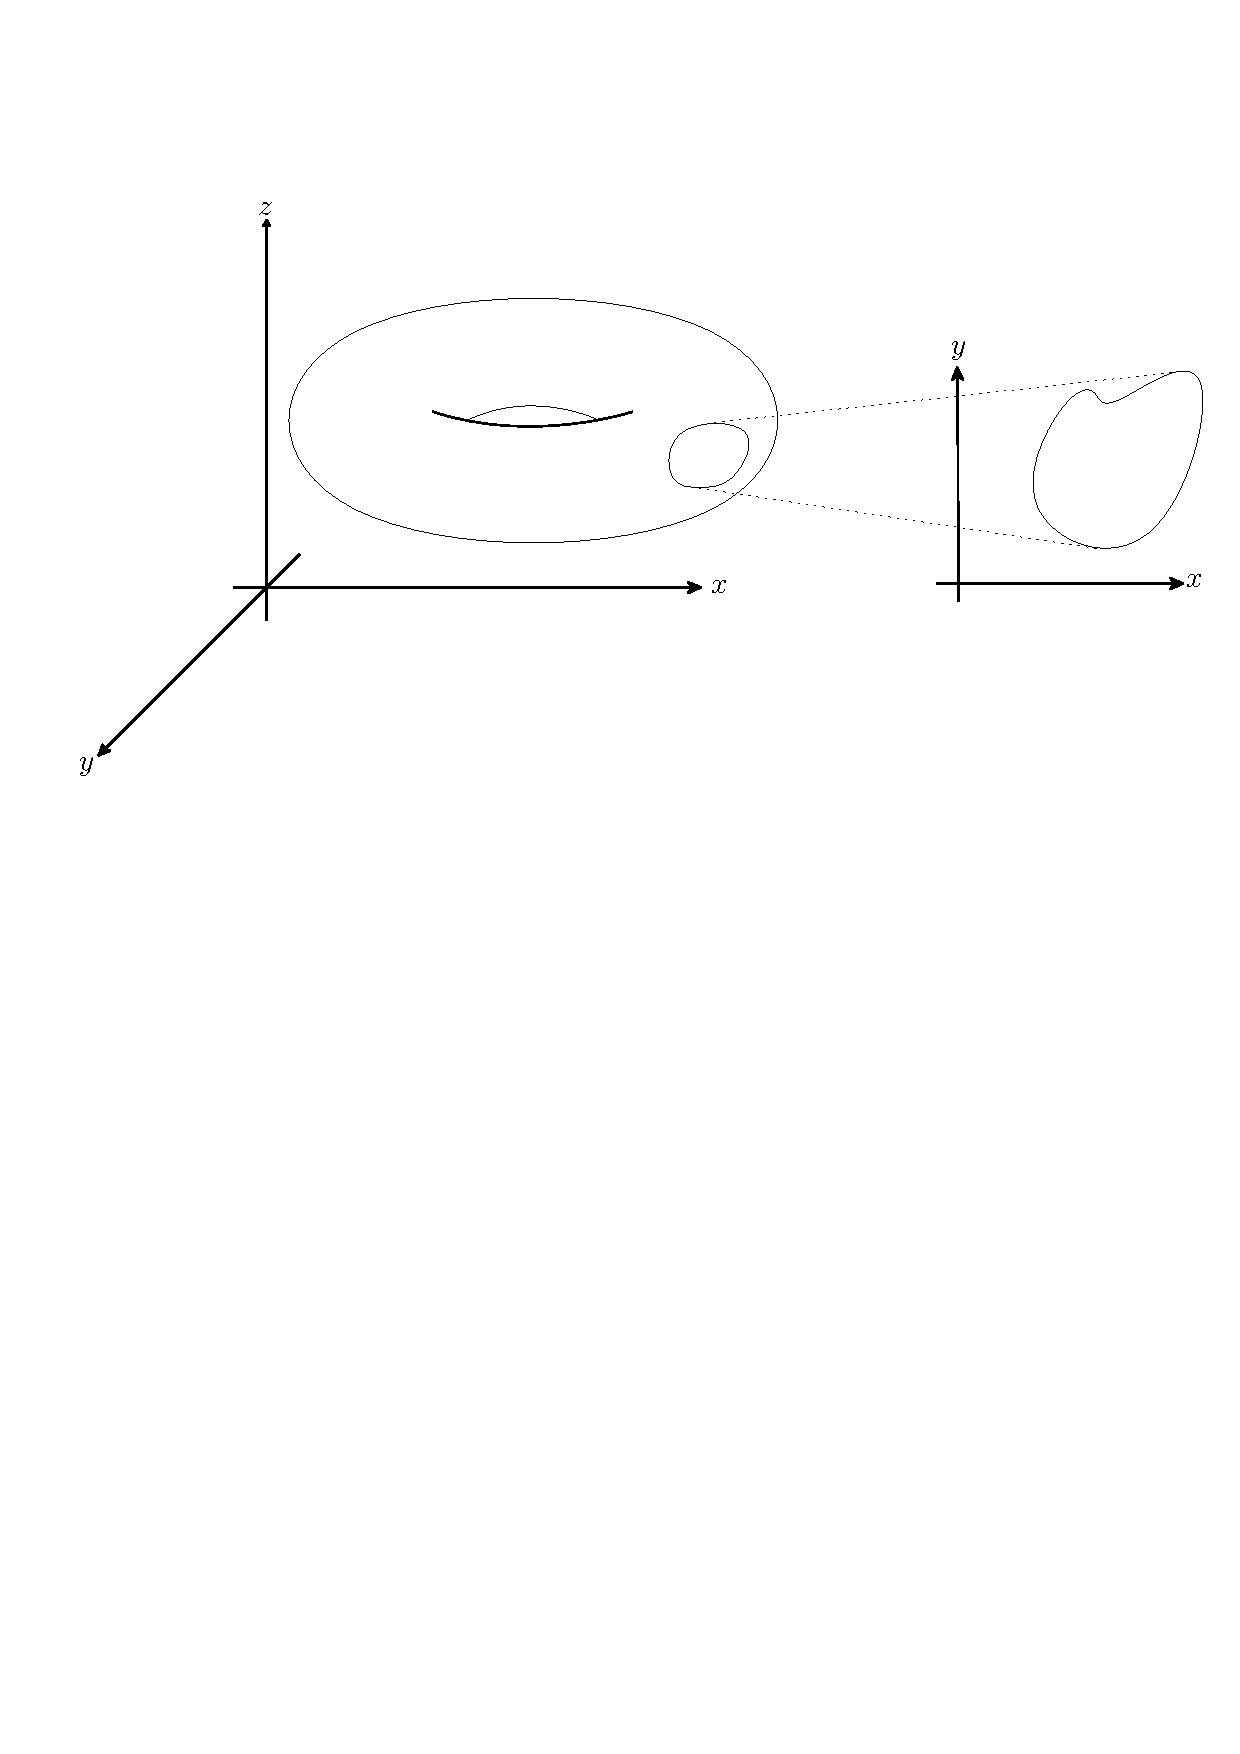
\includegraphics[width=0.713\textwidth]{figures/1_embedded_manifold}
	\caption{A (hyper)surface immersed in $\R^3$}
\end{figure}

In this chapter, symbols referring to $(\overline{M}^{n+1}, \overline{g})$ will have a line on top, otherwise the symbol will refer to $(M^{n}, g)$. In particular, they do not refer to the closure of some set. 


The pullback of the tangent bundle of $\overline{M}^{n+1}$ to
$M^{n}$ is a smooth vector bundle on $M^{n}$:
\begin{align*}
	X^{*}T\overline{M}^{n+1}=T\overline{M}^{n+1}|_{M^n}= \amalg_{p \in M^n} T_p\overline{M}^{n+1}
\end{align*} 

\begin{figure}
	\centering
	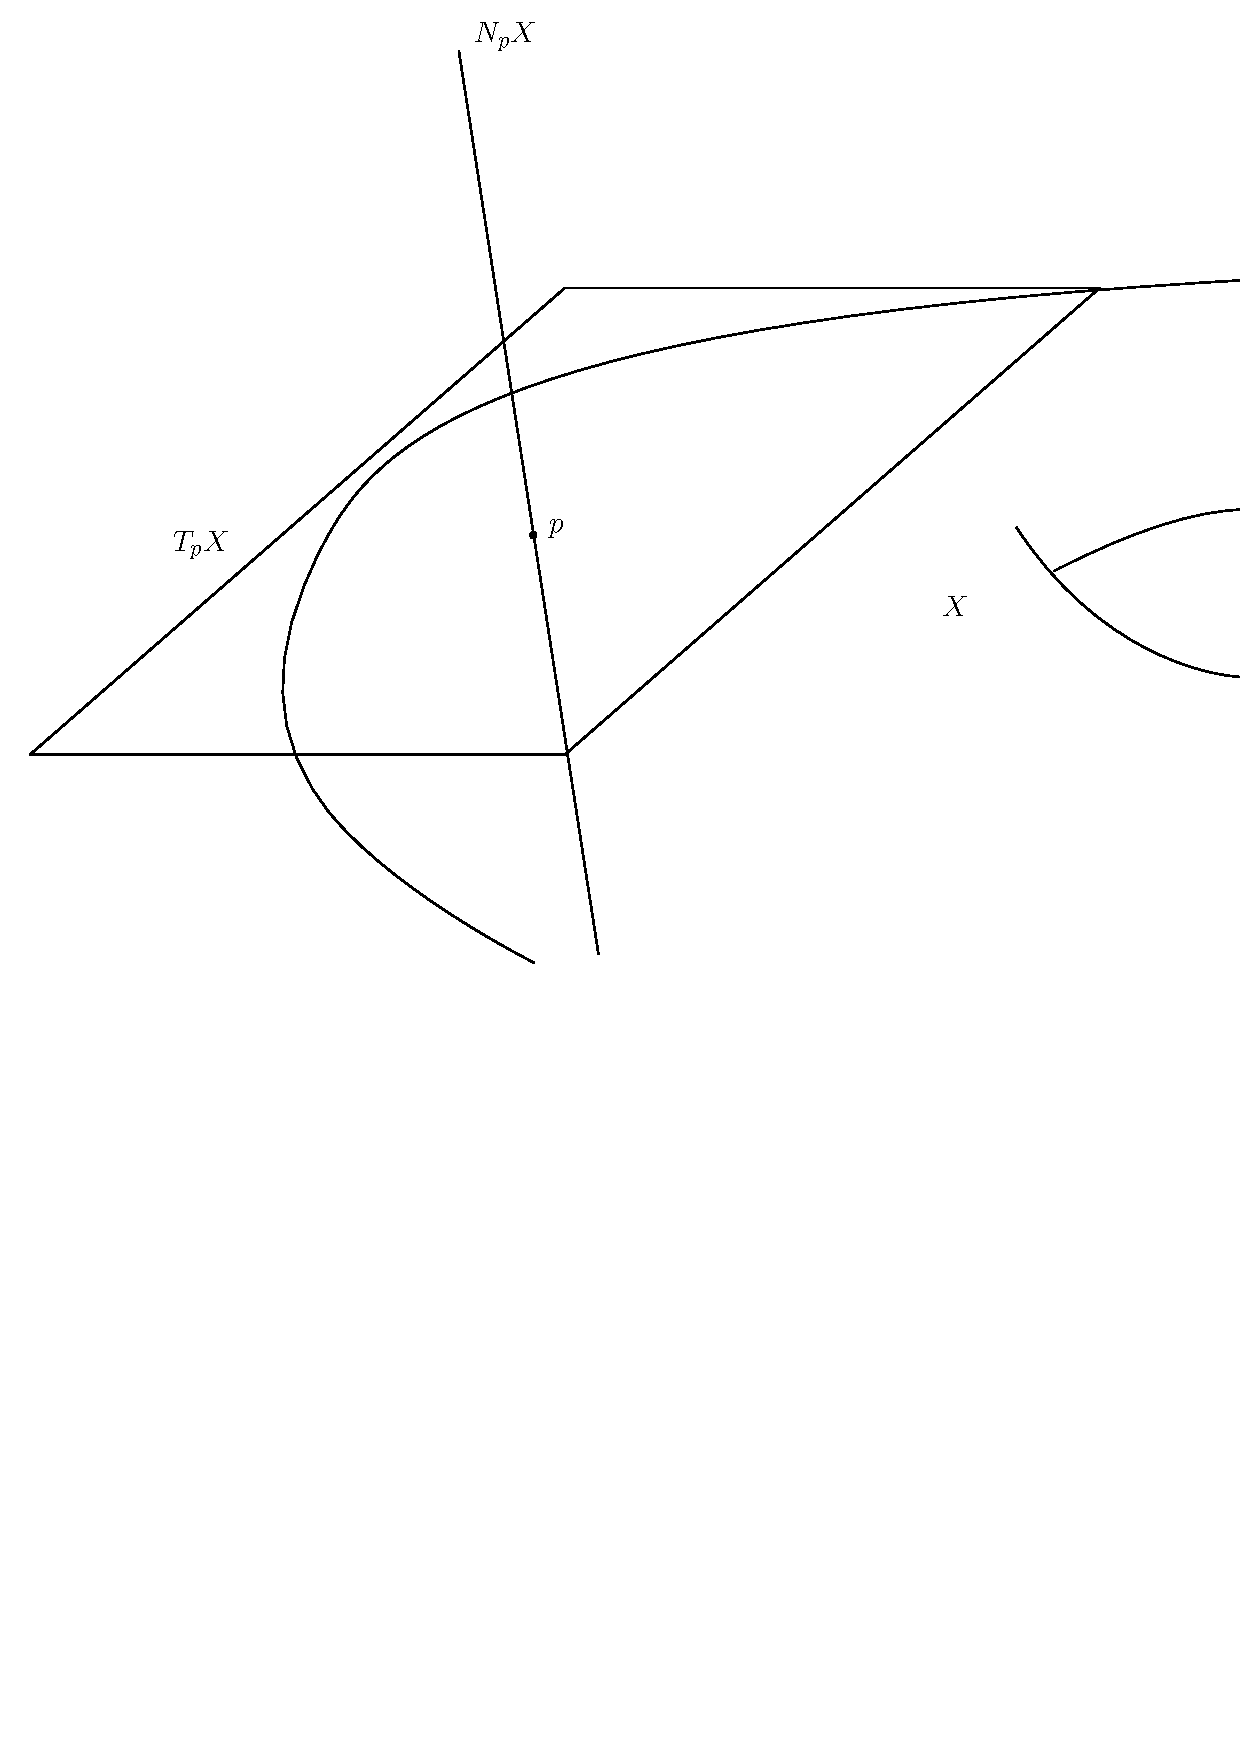
\includegraphics[width=\textwidth]{figures/2_tangent_and_normal_bundles}
	\caption{The tangent and the normal bundle at a point $p$}
\end{figure}


%One of the most important concepts in the geometry of immersed hypersurfaces is the concept of a normal vector field.
The normal vector field $\nu$ is a section of the pullback vector bundle $X^* TM^{n+1}$ on the manifold $M^n$ that is perpendicular to the tangent space of $M^n$ at each point. At each point $p$:
\begin{align*}
	T_p\overline{M}^{n+1}=T_pM^{n}\oplus N_pM^{n}
\end{align*} 
where $N_pM^{n}$ is the normal vector bundle generated by the normal vector. If the manifold is oriented, there is usually a choice we can make on the normal vector: whether we choose to take the inward or outward pointing vector. We will choose the latter through unless otherwise specified. This also allows us to define the tangent and normal projection on $T\overline{M}^{n+1}|_{M^n}$ by taking the two respective components. 

Clearly, taking $\overline{\nabla}$ to be the Levi-Civita connection on $(\overline{M}^{n+1}, \overline{g})$, we can decompose it as:
\begin{align*}
	\overline{\nabla}_v w = (\overline{\nabla}_v w )^\top +  (\overline{\nabla}_v w )^\bot
\end{align*} 

\begin{defin}
	The {\em second fundamental form} is then defined as: 
	\begin{align*}
	 	\mathrm{I\!I} (v, w) =  (\overline{\nabla}_v w )^\bot 	
	\end{align*} 
\end{defin}
It is a bilinear symmetric tensor because $TM^n$ is involutive in $T\overline{M}^{n+1}$ and depends only on the local value of $v$ and $w$ by symmetry. we can therefore write it as
\begin{align*}
	\mathrm{I\!I} (v, w) = -(h_{ij}v^iw^j)\nu
\end{align*} 
for some matrix $A(p)=\{h_{ij}\}$. we can define the principal curvatures of the hypersurface, as the eigenvalues of this matrix.

It is also possible to check that $(\overline{\nabla}_v w )^\top$ satisfies the definition the Levi-Civita connection on $(M^n, g)$, therefore, from its uniqueness:
\begin{align*}
	\nabla_v w &=  (\overline{\nabla}_v w )^\top	\\
	\overline{\nabla}_v w &= \nabla_v w  + \mathrm{I\!I} (v, w) 
\end{align*} 
where $\nabla$ is the Levi-Civita connection on $(M^n, g)$. This result is known as the {\em Gauss Formula}. It has to be noted however that we are implicitly considering tangent vectors that are not in the same space. Indeed, making that more explicit, the formula should be:
\begin{align*}
	\overline{\nabla}_{X_*v} X_* w &= X_* (\nabla_v w)  + \mathrm{I\!I} (v, w) 
\end{align*}

\begin{proposition}
	\textbf{\em (The Weingarten Equation)} If $v, w \in TM^n$ and $\nu \in NM^n$, if one considers the corresponding derivations in $T\overline{M}^{n+1}$ the following equation holds:
	\begin{align*}
			\left\langle \overline{\nabla}_v \nu, w \right\rangle_{\overline{g}} = - \left\langle \nu, \mathrm{I\!I} (v, w) \right\rangle_{\overline{g}}
	\end{align*}
\end{proposition}
\begin{proof}
	As $\left\langle \nu, w \right\rangle_{\overline{g}}\equiv 0$ on $M$, 
	\begin{align*}
		0&=v\left\langle \nu, w \right\rangle_{\overline{g}}\\
		&=\left\langle  \overline{\nabla}_v \nu, w \right\rangle_{\overline{g}} + \left\langle  \nu, \overline{\nabla}_v w \right\rangle_{\overline{g}}\\
		&=\left\langle \overline{\nabla}_v \nu, w \right\rangle_{\overline{g}} + \left\langle \nu, \mathrm{I\!I} (v, w) \right\rangle_{\overline{g}}
	\end{align*}
	applying the Gauss Formula and the fact that $\nabla_v w \in TM^n$ in the last step
\end{proof}
It is also usual to define the associated Weingarten map, which is the linear map between sections of $M$  $s:\Gamma(M)\rightarrow\Gamma(M)$ satisfying:
\begin{align*}
	\left\langle s(v), w \right\rangle_{g} = \left\langle \nu, \mathrm{I\!I} (v, w) \right\rangle_{\overline{g}}
\end{align*}
the linear map $s$ is also known as the {\em shape operator of $M$}. 

Combining this with the formula above, taking into account that it holds for a generic $w \in TM$:
\begin{align*}
	s(v) = -(\overline{\nabla}_v \nu)^\top
\end{align*}


We are going to use these equations in local coordinates, in the form shown below. 
\begin{proposition}
	The above equations in local coordinates are equivalent to the following equations:
	\begin{align}
		\label{Weingarten1} \frac{\partial^2 X^\alpha}{\partial x^i \partial x^j} - \Gamma^k_{ij}\frac{\partial X^\alpha}{\partial x^k}+\overline{\Gamma}^\alpha_{\beta \delta}\frac{\partial X^\beta}{\partial x^i}\frac{\partial X^\delta}{\partial x^k}=-h_{ij}\nu^\alpha \\
		\label{Weingarten2} \frac{\partial \nu^\alpha}{\partial x^i}+\overline{\Gamma}^\alpha_{\beta \delta}\frac{\partial X^\beta}{\partial x^i} \nu^\delta = h_{ij}g^{jl}\frac{\partial X^\alpha}{\partial x^l}
	\end{align} 
	where $\nu$ is the normal unit vector at the point and $A=\{h_{ij}\}$ is the second fundamental form, thus $h_{ij}= \left\langle  \nu, \overline{\nabla}_{\overline{\partial_i}} \overline{\partial_j} \right\rangle_{\overline{g}} $
\end{proposition}
\begin{proof}
	For any connection $\nabla_\cdot$ and any derivations $v=v^i \partial_i$ and $w=w^j \partial_j$:
	\begin{align*}
		\nabla_{v} w = \nabla_{(v^i \partial_i)} (w^j \partial_j) = v(w^k)\partial_k + (v^i w^j \Gamma^{k}_{ij})\partial_k
	\end{align*}
	Let $\partial_1, \dots \partial_n$ be a basis of $TM^n$ at a point, and let $\overline{\partial_i} = X_*\partial_i$, $\overline{\partial_{n+1}}=\nu$.
	Let's consider the Gauss Formula for two generic $\partial_i$, $\partial_j$, using Roman letters for indices varying between $1$ and $n$ and Greek letters for indices varying between $1$ and $n+1$:%, and $\delta^{ij}$ the Kronecker delta:
	\begin{align*}
		\overline{\nabla}_{X_*\partial_i} X_* \partial_j &= X_* (\nabla_{\partial_i} \partial_j)  + \mathrm{I\!I} (\partial_i, \partial_j) \\
		(\overline{\partial_i}(X_*\partial_j)^\alpha) \partial_\alpha + ((X_*\partial_i)^\beta (X_*\partial_j)^\delta \overline{ \Gamma}^{\alpha}_{\beta \delta})\overline{\partial_\alpha} &= X_* (\Gamma^{k}_{ij}\partial_k)  - h_{ij}\nu^\alpha \overline{\partial_\alpha}\\
		%(\overline{\partial_i}(X_*\partial_j)^\alpha) \partial_\alpha + ((X_*\partial_i)^\beta (X_*\partial_j)^\delta\overline{ \Gamma}^{\alpha}_{\beta\delta})\partial_\alpha &= X_* (\Gamma^{k}_{ij}\partial_k)  - h_{ij}\nu^\alpha \overline{\partial_\alpha}\\
		\frac{\partial^2 X^\alpha}{\partial x^i \partial x^j} +\overline{\Gamma}^\alpha_{\beta \delta}\frac{\partial X^\beta}{\partial x^i}\frac{\partial X^\delta}{\partial x^k}&=\Gamma^k_{ij}\frac{\partial X^\alpha}{\partial x^k}-h_{ij}\nu^\alpha
	\end{align*}
	Which is the formula (\ref{Weingarten1}). 
	To get the second formula, first note that $s(v) = -(\overline{\nabla}_v \nu)^\top$. We then compute $-\langle s(\partial_i), \overline{\partial_\alpha}\rangle_{\overline{g}}$:
	\begin{align*}
		\left\langle\overline{\nabla}_{\overline{\partial_i}} \nu, \overline{\partial_\alpha}\right\rangle_{\overline{g}} &= -\left\langle s(\partial_i), \overline{\partial_\alpha}\right\rangle_{\overline{g}}\\
		\left\langle \left(\frac{\partial \nu^\alpha}{\partial x^i}+\overline{\Gamma}^\alpha_{\beta \delta}\frac{\partial X^\beta}{\partial x^i} \nu^\delta \right)\overline{\partial_\alpha}, \overline{\partial_\alpha} \right\rangle_{\overline{g}}&= h_{ij}g^{jl}\frac{\partial X^\alpha}{\partial x^l}
	\end{align*}
	leading to (\ref{Weingarten2}).
	\begin{comment}
	Similarly, taking the Weingarten Equation and the definition of $h_{ij}$:
	\begin{align*}
		h_{ij} &=\left\langle  \nu, \overline{\nabla}_{\overline{\partial_i}} \overline{\partial_j} \right\rangle_{\overline{g}} = - \left\langle  \overline{\nabla}_{\overline{\partial_i}} \nu, \overline{\partial_j} \right\rangle_{\overline{g}}\\
		&= - \left\langle \overline{\partial_i}(\nu^\alpha) \overline{\partial_{\alpha}} + ((\overline{\partial_i})^\beta \nu^\delta \Gamma^{\alpha}_{\beta\delta})\overline{\partial_\alpha}, \overline{\partial_j} \right\rangle_{\overline{g}} \\
		&= - \left\langle  (\frac{\partial \nu^\alpha}{\partial x^i}+\overline{\Gamma}^\alpha_{\beta \delta}\frac{\partial X^\beta}{\partial x^i} \nu^\delta )\overline{\partial_\alpha}, \overline{\partial_j} \right\rangle_{\overline{g}}		
	\end{align*}
	Which leads to (\ref{Weingarten2}) by applying the inverse of the metric $g^{jl}$ to both sides. 
	contenuto...
	\end{comment}
\end{proof}


% The Weingarten equations are important in the study of the local properties of immersed hypersurfaces, for example, the second kind equation relates the normal vector field to the shape operator and can be used to compute the mean curvature of the hypersurface. 

% Another important concept in the geometry of immersed hypersurfaces is the Gaussian curvature. The Gaussian curvature is a scalar valued function that describes the total curvature of the hypersurface at each point. It is defined as the product of the eigenvalues of the shape operator and it is closely related to the sectional curvature of the ambient space.

%There exist many important partial differential equations (PDEs) which stem from the study of immersed hypersurfaces, for example, the minimal surface equation, which is a PDE that describes surfaces with minimal area, can be seen as a geometric condition on the mean curvature of an immersed hypersurface. Likewise, the mean curvature flow is a geometric flow that deforms an immersed hypersurface by moving each point along the normal vector field at that point by an amount proportional to the mean curvature at that point. This flow is important in the study of geometric PDEs and is used to obtain a lot of important results in differential geometry.

% Some other important results useful for the study of PDEs on immersed manifolds are:


%The Gauss-Codazzi equations: These are a set of equations that relate the curvature of an immersed hypersurface to the curvature of the ambient space. These equations are important in the study of geometric PDEs and are used to obtain a lot of important results in differential geometry.

%The Gauss equation: This is an equation that relates the Gaussian curvature of an immersed hypersurface to the sectional curvatures of the ambient space. It is important in the study of the global properties of immersed hypersurfaces.

%The Gauss-Bonnet theorem: This is a theorem that relates the Gaussian curvature of an immersed hypersurface to the topology of the hypersurface. It is important in the study of the global properties of immersed hypersurfaces and is used to prove many important results in differential geometry.

\section{Local representation as a graph}

%A well known result, Dini's Theorem\footnote{also known as Implicit Function Theorem}, states that, given a smooth function $F$ defined on an open subset of the product space $\R^n \times \R^m$, if $F(x,y) = 0$ and the partial derivative matrix of $F$ with respect to $y$ is invertible at a point $(x_0, y_0)$, then there exists an open neighbourhood of $x_0$ in $\R^n$ and a unique smooth function $y = g(x)$ defined on that neighbourhood such that $y_0$ is a regular value of $g$ and $(x, g(x))$ is a smooth solution to the equation $F(x, y) = 0$.

Consequence of the Inverse Function theorem is a powerful result that allows one to locally represent a submanifold of $\R^{n+1}$ as the graph of a smooth function. We provide a version of this theorem below:

\begin{theorem}[Local representation as a graph]
	Let $X^n$ be a submanifold $X^n\subset\R^{n+1}$ and let $x_0\in X$. Then there exists a neighbourhood of $x_0$, $U\subset X^n$, such that $U$ is the graph of a function. 
	Moreover, this function can be of the form 
	\begin{align*}
		f:\pi(U)\subset&\R^n\rightarrow U \\
		U=\{(x_0, \dots, x_n)\in \R^{n+1}&|x_0= f(x_1, ..., x_n)\}
	\end{align*}
	for any of the possible orders of the usual basis for $\R^n$, $(e_0, \dots, e_n)$, as long as $e_0\notin T_xM$, where $\pi(U)$ is the projection on the last $n$ coordinates ($(x_0, \dots, x_n) \mapsto (x_1, \dots, x_n)$). \label{localgraphclassic}
\end{theorem}

A proof of the 2D-case of the version of the theorem can be found in \cite{DoCarmo} which extends naturally to the $n$ dimensional case, with almost no changes. This immediately extends to:

\begin{cor}[Local representation as a graph on the tangent]
	Let $X^n$ be a submanifold $X^n\subset\R^{n+1}$ and let $x_0\in X$. Then there exists a neighbourhood of $x_0$ $U\subset X^n$ and a smooth function $f: T_x X^n\rightarrow \R$ such that any $x_0\in U$ can be expressed as \label{localgraphcorollary}
	\begin{align*}
		x_0= p + f(p) \nu 
	\end{align*}
	where $\nu$ is the vector normal to $T_{x_0} X^n$, for an appropriate point $p\in T_{x_0} X^n$. 
	In other words, every submanifold $X^n\subset\R^{n+1}$ is locally expressible as a graph on its tangent space. 
\end{cor}

\begin{proof}
	By rotation, we may assume $T_x X^n$ orthogonal to $e_1$. Then one can just apply the previous theorem. 
\end{proof}

We will use this later to prove Theorem \ref{localgraph}. 


\section{Some well established results from analysis}

We now include some well known results from analysis which will be useful later. The first result we introduce is the maximum principle.

The maximum principle is a classical result of mathematical analysis, and it is usually introduced in a first course on partial differential equations. It is a fundamental tool in the theory of partial differential equations. It is a statement about the behaviour of solutions to certain types of PDEs and provides a method for obtaining upper and lower bounds on the solutions. The principle states that the maximum and minimum values of a solution to elliptic or parabolic PDE occur on the boundary of the domain unless the function is constant. 

The maximum principle can be used to prove the existence, uniqueness, and regularity of solutions to elliptic and parabolic PDEs. It can also be used to obtain estimates on the behaviour of solutions and to study the asymptotic behaviour of solutions as the domain becomes large. The principle is widely used in many fields of mathematics and physics, such as geometric analysis, mathematical physics, and fluid dynamics. One of the many versions of this well know theorem is this: 

\begin{theorem}[Maximum principle for parabolic equations]\label{maximum_principle}
	Let $\Omega$ be an open, bounded, connected set. Assume $u\in C^2_1(\Omega\times [0, T])\cap C^1(\overline{\Omega}\times [0, T])$. Suppose $u$ satisfies: 
	\begin{align}
		-\frac{\partial u}{\partial t} + \left(\sum_{i, j=1}^n a_{ij}\frac{\partial^2 }{\partial x_i\partial x_j}+\sum_{i}^n b_{i}\frac{\partial }{\partial x_i} + c\right)  u = -u_t + Lu \geq 0 \label{condition_max_principle}
	\end{align}
	where $L$ is an elliptic differential operator, i.e. there exists $\theta>0$ such that $\sum_{i,j=1}^{n} a_{ij}(x, t) \xi_i\xi_j \geq \theta |\xi |^2$ for all $\xi \in \R^n$ and $(x, t) \in \Omega\times[0, T]$. Suppose also that $c\equiv 0$ in $\Omega$. Then: \begin{itemize}
		\item if $u$ attains its maximum in an interior point $(x_0, t_0)\in\Omega\times [0, T]$, then $u$ is constant in $\Omega\times [0, t_0]$.
		\item If, instead, under the same conditions, $u_t- Lu \geq 0$ and attains its minimum in an interior point of $\Omega\times [0, T]$, then $u$ is constant in $\Omega\times [0, t_0]$
	\end{itemize}
\end{theorem}
A proof of this result can be found, for example, in \cite{Evans}. The theorem extends also to situations where the condition holds in a bounded connected region $R\subseteq \Omega \times [0, T]$: in that case, if $u$ attains its maximum in an interior point then $u$ has the same value at any point in $R$ that can be connected to it through a segment going in the backwards direction of time and a "horizontal" line contained in $\Omega$. This version of the theorem can be found for example in \cite{protterweinberger}: 
\begin{theorem}
	Let $u$ satisfy the uniformly parabolic differential inequality (\ref{condition_max_principle}) with $c(x)\leq 0$
	in a region $R_T =\{(x_1,x_2, \dots ,x_n ,t)\in R\vert t\leq T\}$ where $R$ is a non-empty connected open set, and suppose that the coefficients of $L$ are bounded. Suppose that the maximum of $u$ in $R_T$ is $M$ and that it is attained at a point $(x, t)$ of $R_T$. Thus if $(y,s)$ is a point of $R$ which can be connected to $(x,t)$ by a path in $R$ consisting only of horizontal segments and upward vertical segments, then $u(y,s) = M$.\label{maxprincprotterweinberger}
\end{theorem}

Hopf's boundary point lemma is another important classical tool in the study of PDEs that provides a criterion for determining the behaviour of solutions to certain types of elliptic or parabolic PDEs near the boundary of the domain. The lemma states that if one has a solution to some kinds of partial differential inequalities, then the normal derivative of the solution at that point is strictly positive.

It is often used to obtain estimates on the behaviour of solutions near the boundary, and to prove the existence and uniqueness of solutions to boundary value problems. The lemma is named after the German mathematician Eberhard Hopf, who first formulated it in the 1950s. In \cite{protterweinberger} we find the following version of the Hopf's boundary point lemma:

\begin{theorem}
	Let u be a solution to the parabolic inequality 
	\begin{align*}
		-u_t+Lu\geq 0
	\end{align*} 
	with $L$ an elliptic linear differential operator with bounded coefficients such that $c(x)\leq 0$,in a domain $E$, and let $E_t = \{(x, s) \in E | s \leq t\}$. Suppose the maximum $M$ of $u$ is attained at a point $P=(x, t)$ on the boundary $\partial E$. \\
	Assume that a sphere through $P$ can be constructed which is in $E$ such that
	\begin{itemize}\itemsep0em 
		\item tangent to $\partial E$ at $P$
		\item the set of point of its interior $(y, s)$ such that $s\leq t$ lies in $E_s$, 
		\item  $u < M$ in its interior.
	\end{itemize}	
	Also, suppose that the radial direction from the centre of the sphere to P is not parallel to the t-axis. \\
	Then, if $\frac{\partial}{\partial \nu}$ denotes any directional derivative in an outward direction from $E_s$ , we have
	\begin{align*}
		\frac{\partial u}{\partial \nu} > 0
	\end{align*}
	at P.\label{HopfBPL}
\end{theorem}

\begin{figure}
	\centering
	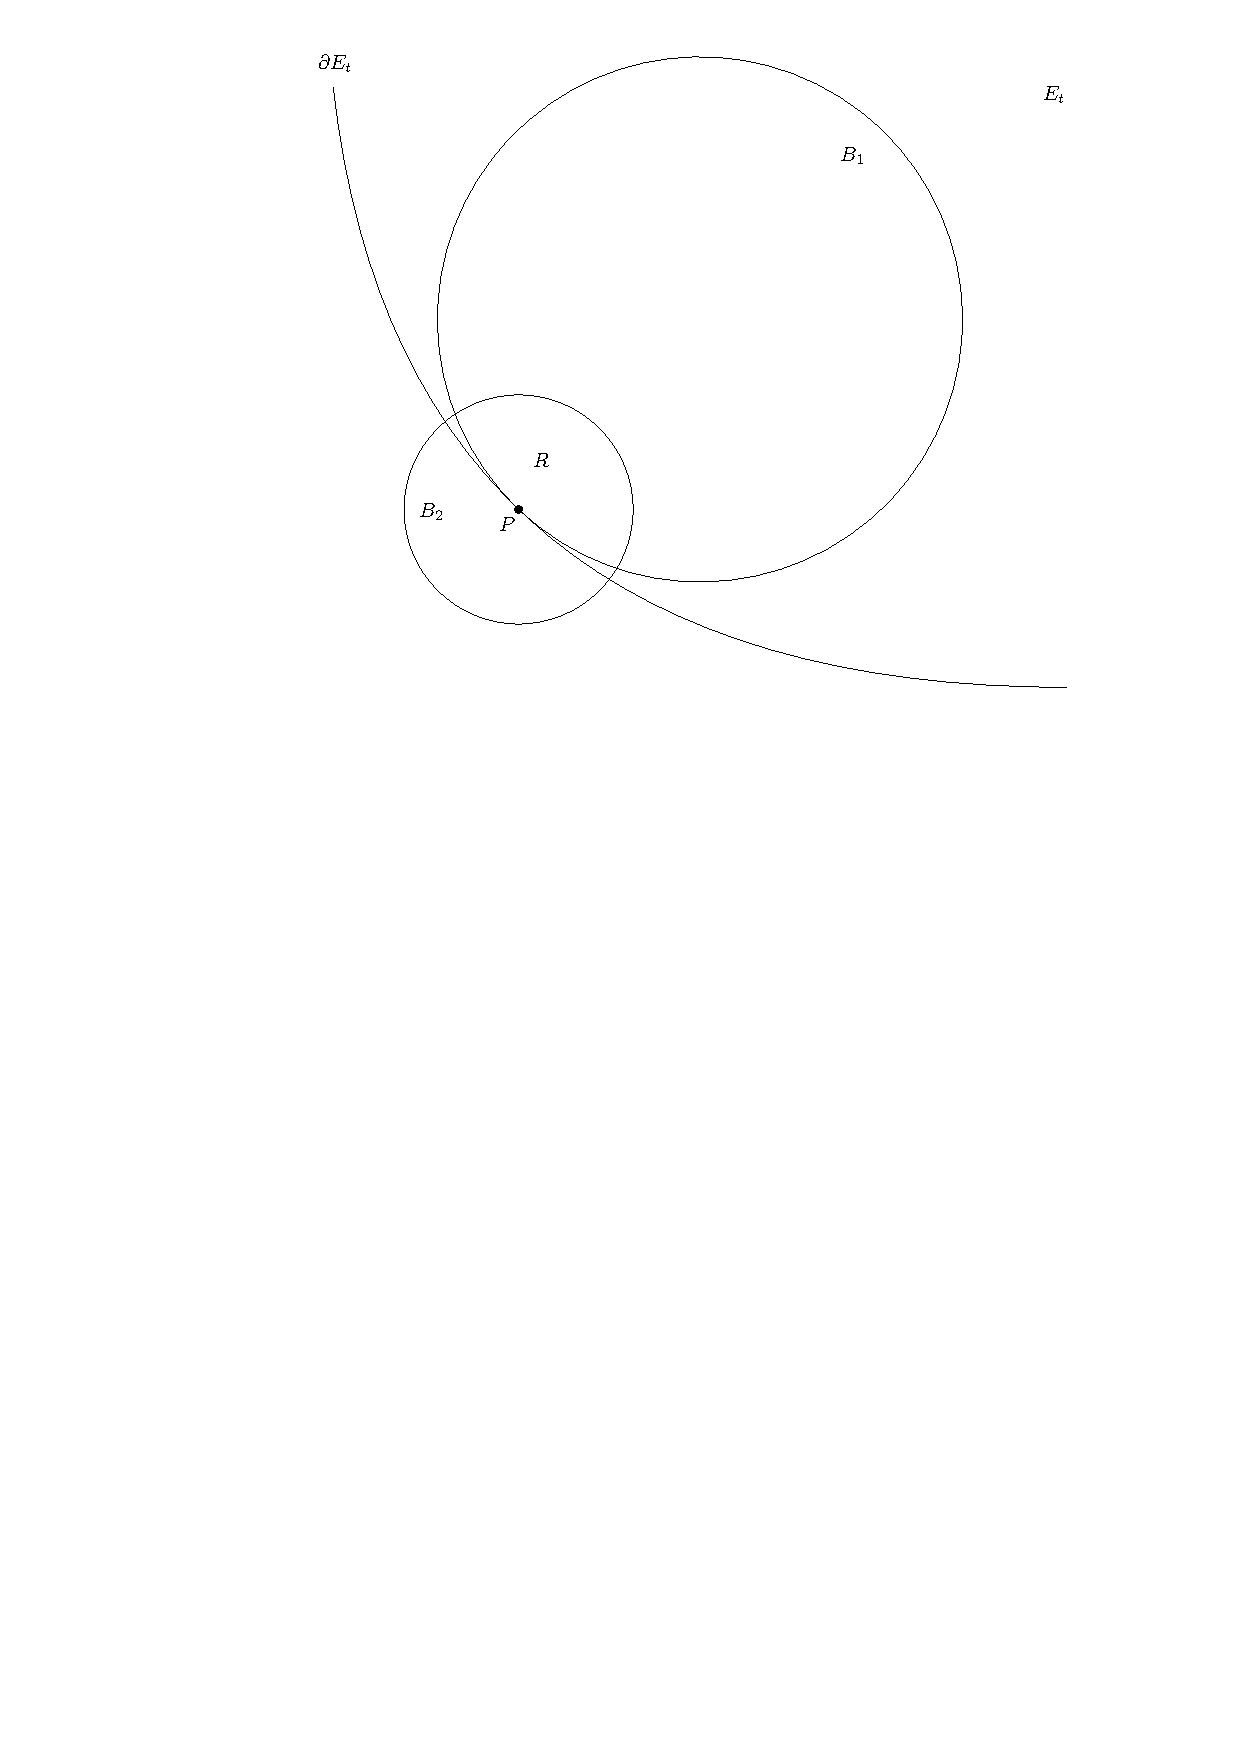
\includegraphics[width=\textwidth]{figures/3_Hopf_boundary_point_lemma}
	\caption{The setup in the proof at time $t$ when there are two space dimensions. The region $R$ also extends for times $s<t$ between the two spheres. The centre of $B_1$ can have time-coordinate different from $t$ if the domain $E$ is not ``straight" in the time direction.}
\end{figure}
\begin{proof}
	Let the sphere through $P$ be $B_1$. We may construct a smaller sphere $B_2$ centred at $P$. Let now:
	\begin{align*}
		S_1 &= \partial B_1 \cap  B_2 \cap E_t, \\
		S_2 &= B_1 \cap \partial  B_2 \cap E_t, \mathrm{ and} \\
		S_3 &= B_1 \cap  B_2 \cap \partial E_t= B_1 \cap  B_2 \cap \{(x, s) \in E | s=t\}.
	\end{align*}
	The three sets satisfy $S_1\cup S_2 \cup S_3 = \partial (B_1 \cap  B_2 \cap E_t)$, we may call this region $R=B_1 \cap  B_2 \cap E_t$. Without loss of generality, potentially taking a smaller sphere $B_1$, we may assume that $u<M$ on $B_1$ except at $P$. As $R \subset B_1$, we also get  $u<M$ on $R$. 
	We may thus conclude that: 
	\begin{itemize}\itemsep0em 
		\item  $u<M$ on $R$ except at $P$
		\item  $u\leq M-\delta$ on $S_2$ for a sufficiently small $\delta>0$
		\item  $u=M$ at $P$.
	\end{itemize}	
	Now, let the centre of $B_1$ be $Q=(z, t_0)$ and let $r$ be its radius. we can now introduce the function	
	\begin{align*}
		v(y, s) = exp \left(-\alpha(s-t_0)^2-\sum_{i=1}^n\alpha(y_i-z_i)^2\right) - exp\left(-\alpha r^2\right)
	\end{align*}
	This function is such that $v(y, s)=0$ if $(y, s)\in S_1$ - including  $v(x, t)=0$, as there the first term is $e^{-\alpha r^2}$, and $v(y, s)>0$ in the interior of $B_1$.  \\
	Thus, in the region $R$, $v(y, s)\geq0$ and has a minimum point at the boundary on $(x, t)$, where  $v(x, t)=0$.
	
	We can also compute $Lv$. After some calculation, we get that 
	\begin{align*}
		Lv = 2 \alpha e^{\left(-\alpha(s-t_0)^2-\sum_{i=1}^n\alpha(y_i-z_i)^2\right)}[2\, \alpha\, (y-z&)^t A (y-z) +\\
		+&\sum_{i}^n[ b_i (y_i-z_i)+a_{i,i}]+(s-t)]
	\end{align*}
	where $A$ is the matrix of the $a_{i,j}$. In particular, one can choose an $\alpha$ large enough, so that $Lv>0$ in $R\cup \partial R$.
	
	We can thus introduce $w=u+\varepsilon v$. As both $Lu$ and $Lv$ are positive in $R$, $Lw>0$ in $R$. We can also choose $\varepsilon$ small enough so that $w<M$ on $S_2$. Also, as $v=0$ on $S_1$, $w<M$ on $S_1$ except at $P$, and $w=M$ at $P$.
	
	Therefore, we can apply the Strong Maximum Principle \ref{maxprincprotterweinberger} to the region $R$ to conclude that the maximum of $w$ in $R$ is attained at $P$. Therefore:
	\begin{align*}
		\frac{\partial w}{\partial \nu}=\frac{\partial u}{\partial \nu}+\varepsilon\frac{\partial v}{\partial \nu}\geq0
	\end{align*}
	But:
	\begin{align*}
		\frac{\partial v}{\partial \nu}=\nu \cdot n\frac{\partial v}{\partial R} = - 2\nu \cdot n \alpha Re^{-\alpha R}<0
	\end{align*}
	Where $n$ is the vector orthogonal to the sphere $S_1$. Therefore, one must have:  
	\begin{align*}
		\frac{\partial u}{\partial \nu}>0
	\end{align*}
	as we wanted.
\end{proof}
\begin{oss}\label{removecpositive}
	\em If $c(x)$ is now just bounded, we can consider, instead of $u$, $v= u e^{-\lambda t}$, thus, by change of variables 
	\begin{align*}
		-v_t+Lv-\lambda v \geq 0
	\end{align*}
	whenever $-u_t+Lu\geq 0$, and we can chose $\lambda$ large enough such that $c(x)-\lambda<0$ and thus we can remove the hypothesis $c(x)\leq0$ in both theorems when $c$ is bounded. 
\end{oss}

\section{Applying the maximum principle to non-linear PDEs}
\label{non linear pde parabolic section}
Following the approach in \cite{protterweinberger}, it is easy to show that the maximum principle \ref{maxprincprotterweinberger} and Hopf's boundary point lemma \ref{HopfBPL} can be applied - appropriately adapted - in some non-linear settings.  Firstly, we must clarify what we mean by parabolic non-linear problem. 
\begin{defin}\label{nonlinearpde}
	A differential non-linear problem in the form 
	\begin{align}
		Lu= F\left(t, x, v, \frac{\partial v}{\partial x_i} , \frac{\partial^2 v}{\partial x_i \partial x_j}\right)-v_t = f(x, t)\label{nonlinearexample}
	\end{align} 
	given a smooth $F$ is {\em parabolic with respect to a function $v$} if for any real vector $\xi$
	\begin{align*}
		\sum_{i, j=1}^n F_{ij}\xi_i\xi_j >0
	\end{align*} 
	where $F_{ij}$ are the derivatives of $F$ with respect to $\frac{\partial^2 v}{\partial x_i \partial x_j}$. 
\end{defin}
\begin{comment}
	First, let's introduce an easier example from \cite{GidasNirenberg}: 
	Suppose that $u$ solves:
	\begin{align}
		u_t-L u+f(u)=0 \label{non-linear}
	\end{align}
	For an elliptic operator $L$, and where $u_t=\frac{\partial u}{\partial t}$. We note that this differs from the usual parabolic equation because here $f$ depends from the solution $u$, potentially in non-trivial ways, making the equation non-linear. 
	If a solution exists, and $f$ is a $C^1$ function, by the theorem of the mean, at any point $x$ in the domain of $u$ we can find a function $\xi(x)$ such that
	\begin{align*}
		f'(\xi(x))&=\frac{f(u(x))-f(0)}{u(x)-0}\\
		f'(\xi(x))u&=f(u(x))-f(0)
	\end{align*} 
	If $u$ solves (\ref{non-linear}), and if $f(0)\leq0$, then 
	\begin{align*}
		u_t-L u+f(u)-f(0) &\geq 0\\
		u_t-L u+ f'(\xi(x))u&\geq 0 \\
		u_t-L u+ c(x)u&\geq 0
	\end{align*}
	Hence the function $u$ is the super-solution to a (different) linear parabolic partial differential equation and hence we can apply the maximum principle \ref{maxprincprotterweinberger} and Hopf's boundary point lemma \ref{HopfBPL} to solutions of (\ref{non-linear}) as long as the other hypothesis apply to $c(x)$. 
\end{comment}
\begin{figure}
\centering
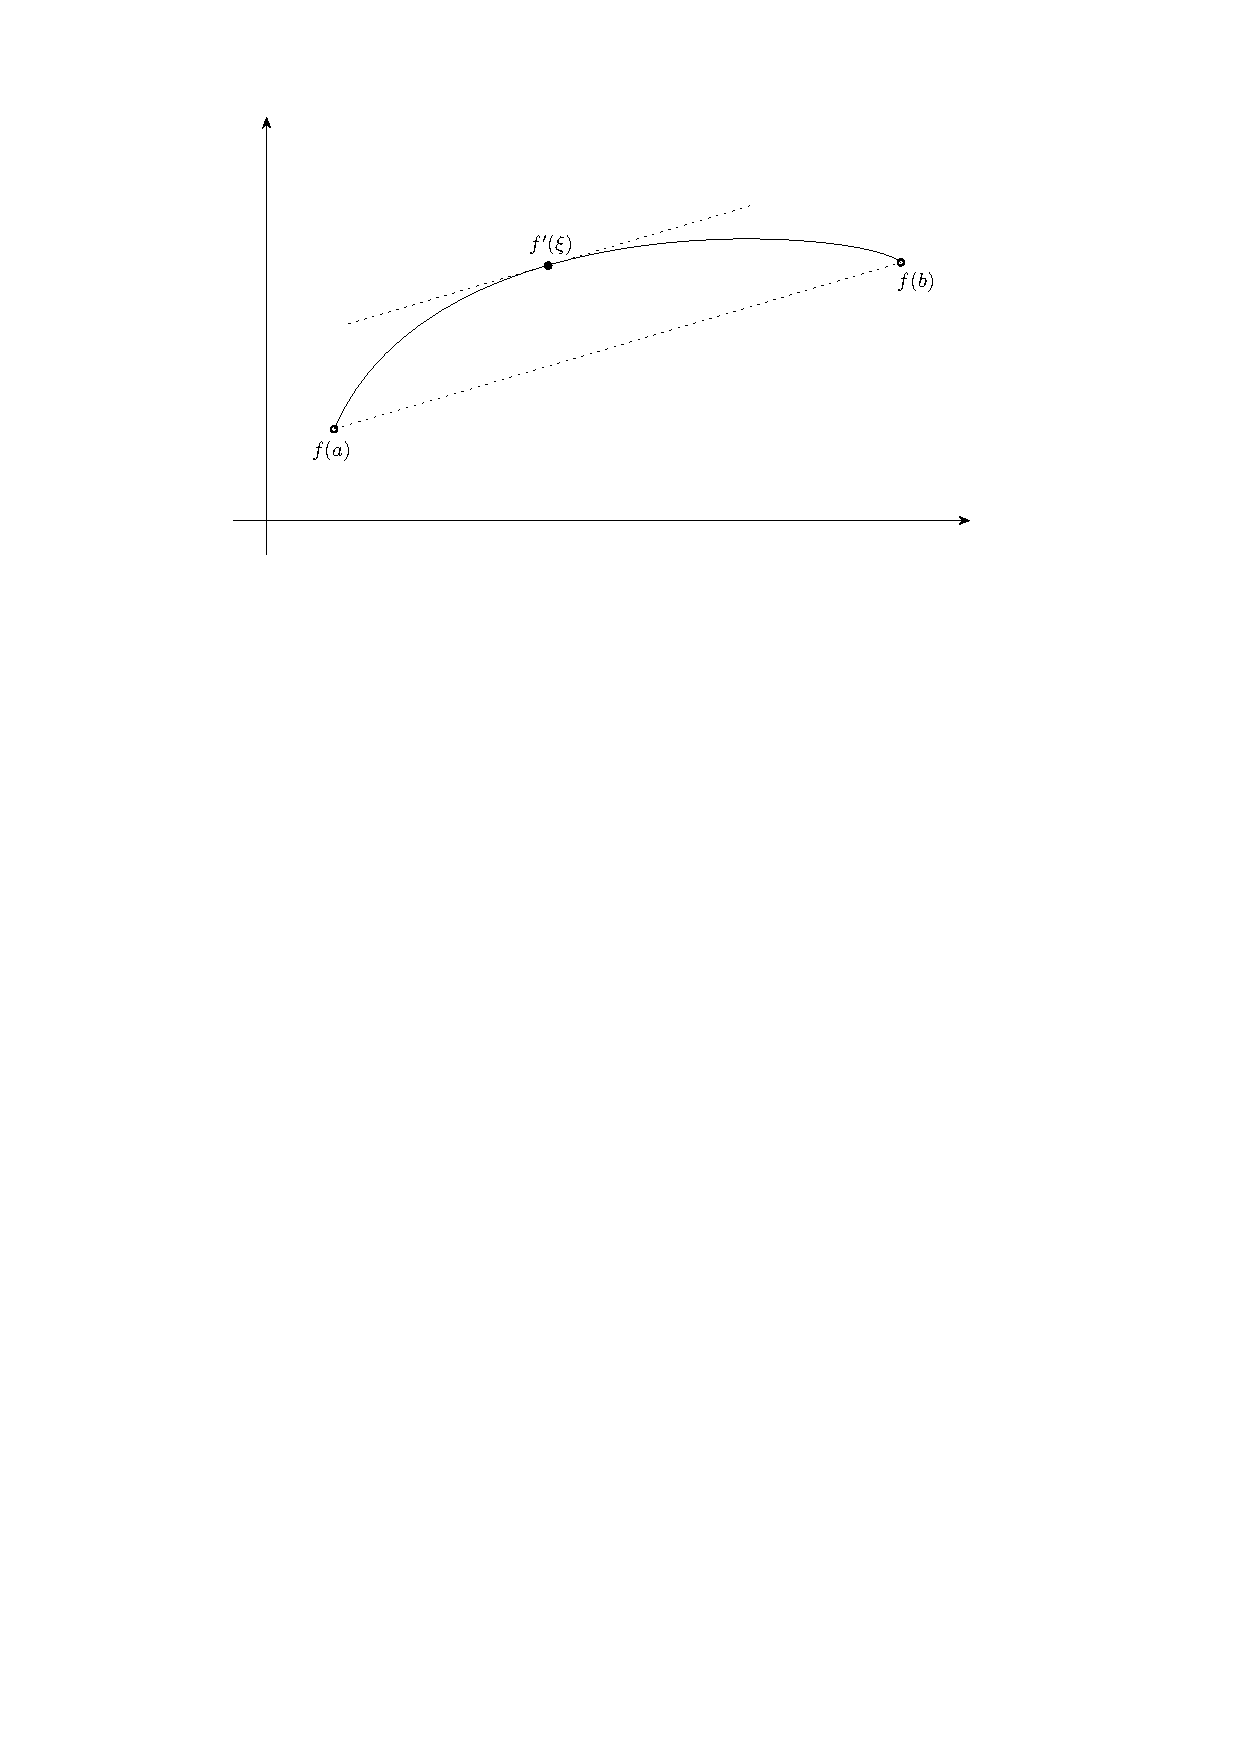
\includegraphics[width=0.713\textwidth]{figures/4_Lagrange_theorem}
\caption{In one dimension, Lagrange's theorem states that given a smooth function $f$ on an interval $[a, b]$, there exists a $\xi$ such that $f(b)-f(a) = f'(\xi) (b-a)$.}
\end{figure}
Secondly, we remind the reader of the following generalized version of the theorem of the mean, a.k.a. Lagrange's theorem:
\begin{theorem}[Lagrange's theorem]
	Given a convex open set $U\subseteq \R^n$ and a real function $F \in C^1(U)$, and given to points $x, y$ in $U$, there exists a point $z$ in the segment connecting $x$ and $y$ such that 
	\begin{align*}
		F(y)-F(x) =\left\langle \nabla F(z), (y-x) \right\rangle 
	\end{align*}
\end{theorem}
Suppose that we have a solution to a non-linear parabolic problem $v$, i.e. $v$ solves (\ref{nonlinearexample}):
\begin{align*}
	Lv= F\left(t, x, v, \frac{\partial v}{\partial x_i} , \frac{\partial^2 v}{\partial x_i \partial x_j}\right)-v_t = f(t, x)
\end{align*}
for a non-linear elliptic operator $L$ in some region $E$, where we assume that $F(t, x,  a, b_i, c_{i,j})$ is a given $C^1$ function. Suppose also that there is a $w$ which is a solution of the corresponding differential inequality:
\begin{align*}
	Lw= F\left(t, x, w, \frac{\partial w}{\partial x_i} , \frac{\partial^2 w}{\partial x_i \partial x_j}\right)-w_t \leq f(t, x)
\end{align*}
One can then consider $u = v-w$, and by combining the above we get: 
\begin{align*}
	\left( F\left(t, x, v, \frac{\partial v}{\partial x_i} , \frac{\partial^2 v}{\partial x_i \partial x_j}\right) - F\left(t, x, w, \frac{\partial w}{\partial x_i} , \frac{\partial^2 w}{\partial x_i \partial x_j}\right)\right)-u_t \leq 0
\end{align*}
Now, we can apply Lagrange's theorem to $F$ to get 
\begin{align*}
	\tilde{L}u= \left\langle \left(\frac{\partial F}{\partial a},\frac{\partial F}{\partial  b_i},\frac{\partial F}{\partial c_{i,j}} \right)(\xi(t, x)), \left(u, \frac{\partial u}{\partial x_i} , \frac{\partial^2 u}{\partial x_i \partial x_j}\right) \right\rangle-u_t \leq 0
\end{align*}
for a fixed $\xi(t, x) = \theta(t,x) v(t,x)  +  (1-\theta(t,x)) w(t,x) $, $\theta \in [0, 1]$.


Thus, the difference $u$ of two sub-solutions to a non-linear differential problem is a sub-solution to a (different) \textit{linear} parabolic problem, as the derivatives of $F$ and $\xi$ do not depend on $u$ ($\xi$ can be chosen a-priori).

%An equivalent condition for a nonlinear problem to be parabolic is that for any real vector $\xi$
%\begin{align*}
%	\sum_{i, j=1}^n F_{ij}\xi_i\xi_j >0
%\end{align*} 
%where $F_{ij}$ are the derivatives of $F$ with respect to $\frac{\partial^2 v}{\partial x_i \partial x_j}$. 
We can thus see that this new problem must be parabolic, because by definition \ref{nonlinearpde} the matrix whose entries are the second order derivatives must be positive definite, and apply the maximum principle and the Hopf's boundary point lemma to $u$. This can allow us to state the following two results which we will be using later:

\begin{proposition}[Maximum principle for parabolic non-linear differential equations]
	\label{firstapplication}
	Suppose we have two solution $v$ and $w$ on the interval $[0, T]$ with different values at $t=0$ to the same non-linear differential equation (\ref{nonlinearexample}) on an bounded open set $\Omega$, parabolic at $v$, $w$ and the functions between them. Suppose also that $F$ is smooth on  $\overline{\Omega}$. Then, if $v>w$ in the interior of $\Omega$ at $t=0$ and $v\geq w$ on $\partial\Omega$,  $v>w$ for all $t\in[0, T]$ in the interior of $\Omega$.
\end{proposition}

\begin{proof}
	$u=v-w\geq 0$ is a solution of a parabolic \textit{linear} differential equation, where the term independent of $u$ is bounded. Furthermore, if we take $c(x, t)$ it must be bounded by compactness. At $t=0$, $u>0$ in the interior of $\Omega$. If, at an interior point $x$, $v=w$ at a certain time $t=\tau$, $u(\tau, x)=0$, and thus $u$ is not constant. However, it attains minimum ($u=0$) at an interior point, thus by Theorem \ref{maximum_principle} it must be constant, a contradiction. 
\end{proof}

\begin{proposition}[Hopf's boundary point lemma for parabolic non-linear differential equations]
	\label{secondapplication}
	Suppose we have two solution $v$ and $w$ with different starting values to the same  non-linear differential equation (\ref{nonlinearexample}), parabolic at $v$, $w$ and the functions between them, in a domain $\Omega$. Suppose also that $F$ is smooth on  $\overline{\Omega}$. Let $u=v-w$ and suppose that the maximum of $u$ is attained at the point $P$. Furthermore, assume that the conditions on the shape of the region $\Omega$ from theorem \ref{HopfBPL} hold. Then, 
	\begin{align*}
		\frac{\partial u}{\partial \nu}(P) >0
	\end{align*}
	where we take $\nu$ as the normal to $\partial\Omega$.
\end{proposition}

\begin{proof}
	$u$ is a solution of a parabolic \textit{linear} differential equation, where  $c(x, t)$ is bounded by compactness. We can then apply Theorem \ref{HopfBPL} to $v$ (see also remark \ref{removecpositive}).
\end{proof}
\chapter{The Alexandrov Moving Planes Method}


\section{Reflections on spheres and hyperbolic spaces}	
\label{reflections definitions}

In what follows, we will focus on manifolds embedded in spaces which have constant sectional curvature. Constant curvature manifolds are classified into three types based on the sign of the curvature:
\begin{itemize}
	\item \textbf{Positive curvature}: \textit{Spherical geometry}, where the curvature is positive and the manifold locally resembles a sphere (e.g., the standard sphere $\mathbb{S}^n$).
	\item \textbf{Zero curvature}: \textit{Flat geometry}, where the curvature is zero and the manifold locally resembles Euclidean space $\mathbb{R}^n$.
	\item \textbf{Negative curvature}: \textit{Hyperbolic geometry}, where the curvature is negative and the manifold locally resembles hyperbolic space $\mathbb{H}^n$.
\end{itemize}

As in \cite{italiani}, we will use the symbol $\mathbb{M}^n$ to indicate a Riemannian manifold that can be replaced by any one of  $\mathbb{S}^n$, $\mathbb{R}^n$ or $\mathbb{H}^n$: the $n$-dimensional sphere, Euclidean plane or Hyperbolic space respectively. 

We will also use use the symbol $\mathbb{M}^n_+$ to indicate a Riemannian manifold that can be replaced by $\mathbb{S}^n_+$, $\mathbb{R}^n$ or $\mathbb{H}^n$: the $n$-dimensional hemisphere, Euclidean plane or Hyperbolic space, respectively.

We will not be considering other ambient spaces, which can be obtained through quotients from the three cases above. 


\begin{defin}
	$\mathbb{H}^n$ is the {\em $n$-dimensional hyperbolic plane}. We can define it as the half space $\{x\in \R^n|x_n > 0\}$ with the Riemannian metric
	\begin{align*}
		g_x=\frac{1}{x_n^2} \langle\cdot, \cdot \rangle
	\end{align*}
	where $\langle\cdot, \cdot \rangle$ is the Euclidean dot product on $\R^n$
\end{defin}


\begin{oss}
	\em This is not the only way we could define the hyperbolic space $\mathbb{H}^n$. Another alternative is taking the $n$-dimensional disc $D^n = \{x\in \R^n|\lVert x \rVert  < 1 \}$ with the Riemannian metric 
	\begin{align*}
		g_x=\frac{4}{(1-\lVert x \rVert^2)^2} \langle\cdot, \cdot \rangle
	\end{align*}
	where $\langle\cdot, \cdot \rangle$ is the Euclidean dot product on $\R^n$.
\end{oss}

\begin{figure}
	\centering
	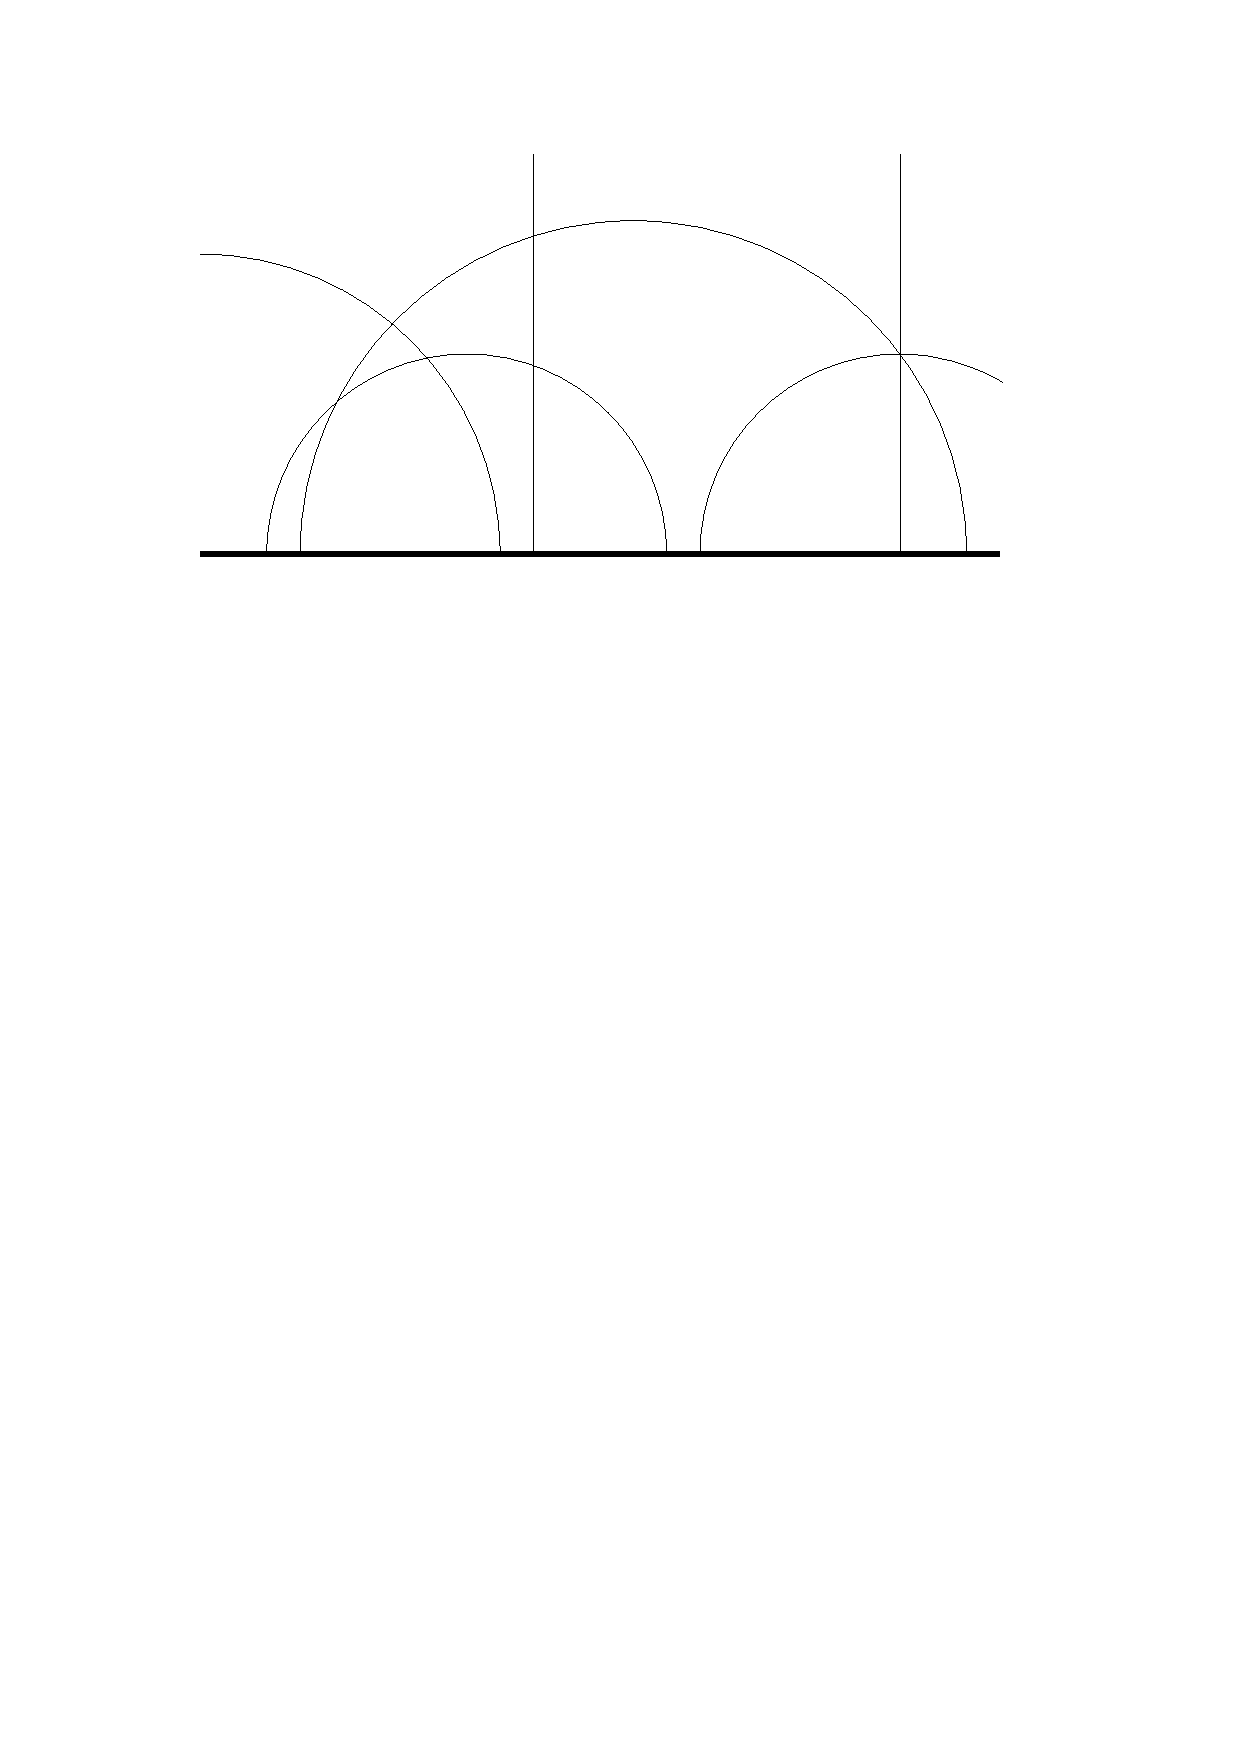
\includegraphics[width=\textwidth]{figures/5_geodesics_hyperbolic_plane}
	\caption{On the half-space model of $\mathbb{H}^n$, geodesics are half lines parallel to the $x_n$ axis and circumferences with centre on the $x_n=0$ hyperplane (see \cite{LeeRiemannian2ndEd}).}
\end{figure}
\begin{oss}
	\em Let $\mathbb{S}^n \setminus \{P\}$ be the standard $n$-dimensional unitary sphere minus a point, with the standard induced Euclidean metric. Through stereographic projection it is isometric to $\R^n$ with metric:
	\begin{align*}
		g_x=\frac{4}{(1+\lVert x \rVert^2)^2} \langle\cdot, \cdot \rangle
	\end{align*}
	where $\langle\cdot, \cdot \rangle$ is again the Euclidean dot product on $\R^n$.
\end{oss}


\begin{oss}
	\em The models above have curvature $\pm 1$. For other values of the curvature one has to consider the following Riemannian metrics
	\begin{itemize}
		\item for the half-space model of hyperbolic space:
		\begin{align*}
			g_x=\frac{R^2}{x_n^2} \langle\cdot, \cdot \rangle
		\end{align*}
		\item for the Poincaré ball model of hyperbolic space one has to take the disk with radius $R$ and:
		\begin{align*}
			g_x=\frac{4 R^4}{(R^2-\lVert x \rVert^2)^2} \langle\cdot, \cdot \rangle
		\end{align*}
		\item For the stereographic projection of a sphere with radius $R$:
		\begin{align*}
			g_x=\frac{4R^4}{(R^2+\lVert x \rVert^2)^2} \langle\cdot, \cdot \rangle
		\end{align*}
	\end{itemize}
\end{oss}

We will now define reflections in $\mathbb{M}^n$. This is relatively straightforward of $S^n$ and a bit more involved for $\mathbb{H}^n$. The ingredients that we need are three: a geodesic, a family of hyperplanes associated to it, and reflections about those. The first one is easy, just take any point and any direction to get a geodesic. Then, at each point on the geodesic, there is an orthogonal totally geodesic hyperplane passing through that point: this is the family we consider. Finally, for each of these hyperplanes there is a reflection about it, which we can describe also mapping the hyperplanes into each other. While this could certainly be done in a more straightforward way compared to the approach we will follow, as we do not really need to know at this stage about what happens to the other planes in the family, and therefore we could just define a reflection about a plane and be satisfied. Using a heavier notation at this stage, however, will make it easier to introduce the moving planes method later.

We will now describe these choices for each ambient space in greater detail:

\begin{itemize}	
	\item On $\R^n$ we can choose any straight line as a geodesic, the hyperplanes orthogonal to it as the associated family, and use the usual reflections.  
	\item On  $S^n$, reflections are those induced by $\R^{n+1}$ when the fixed plane passes through the origin. Each one can be identified by vector orthogonal to the plane we chose. Each hyperplane through the origin in $\R^{n+1}$ defines a $(n-1)$-sphere through intersection with $S^n$. What we want to consider are reflections about $n$-planes through the origin in $\R^{n+1}$ orthogonal to a given geodesic of an immersed copy of $S^n$. 	
	To build an analogy between $S^n$ and $\mathbb{H}^n$, we can parametrize each point in $S^n_+$ in the following way, which will be useful when dealing with both at the same time: 
	\begin{itemize}
		\item choose a point $O$ and a direction $v\in T_O S^n$, and consider the geodesic $\gamma_v$ such that $\gamma_v (0) = O$ and $\dot{\gamma_v} (0) = v$. Assume that $\gamma$ is parametrised by arc-length. 
		\item Consider the $(n-1)$-sphere $\pi_0$ passing through $\gamma_v(0)$ and orthogonal to  $\dot{\gamma_v}(0)$. One can rotate that sphere along the geodesic $\gamma_v$ so that it touches each point in $S^n_+$. We will call the sphere passing through $\gamma_v(t)$ $\pi_{v, t}$. Each point $x$ is in a unique $\pi_{v, t}$.
		\item We can then assign to each point in $S^n_+$ a unique couple of coordinates $(x, t)$, where $x$ is the coordinate in $S^{n-1}\cap S^n_+$ when rotating it back to $\pi_0$, and $t$ is the unique $t$ such that the point is in $\pi_{v, t}$.
	\end{itemize}
	Observe that a reflection about $\pi_{v, s}$ is $(x, t) \mapsto (x, 2s-t)$. This can be either taken as a definition (while being careful dealing with points in the hemisphere opposite to $O$ having ambiguous coordinates) or as a consequence of considering the aforementioned reflection induced on $S^n$ by $\R^{n+1}$ about a plane through the origin. 
	\item On $\mathbb{H}^n$ we can also take a similar construction: 
	\begin{itemize}	
		\item As a first step, choose a point a point $O \in \mathbb{H}^n$. $\mathbb{M}^n$ is a homogeneous space, so the construction does not depend on the choice we make.
		\item Choose any direction in $v\in T_O\mathbb{H}^n$ and consider the geodesic $\gamma_v: \R \rightarrow \mathbb{H}^n$ satisfying $\gamma_v (0) = O$ and $\dot{\gamma_v} (0) = v$. Assume that $\gamma$ is parametrised by arc-length. 
		\item Consider the hyperplane $\pi_0$ passing through $\gamma_v(0)$ and orthogonal to  $\dot{\gamma_v}(0)$. Then consider the 1-parameter group of isometries of $\mathrm{H}^n$ such that $g_t(\gamma_v (0) )=\gamma_v (t) $ and such that the curves $t \mapsto g_t(x)$ are orthogonal to $\pi_0$ for each $x\in \pi_0$. This allows us to assign to each point in $\mathrm{H}^n$ coordinates $(x, t)$ where $x\in\pi_0$ and $t\in \R$.  
		\item consider now any hyperplane  $\pi_t$ passing through $\gamma_v(t)$ and orthogonal to  $\dot{\gamma_v}(t)$. The reflection fixing $\pi_t$ will be the one given by the formula $(x, t)\mapsto (x, 2s-t)$.
	\end{itemize}
	Through rotations and translations it is possible to assume without loss of generality that the point we chose is $e_n$ and the direction is $e_1$ (assuming the half-space model in the definition above). We can do this because $\mathbb{H}^n$ is frame-homogenous (which means that we can move isometrically any point into any other and any direction into any other, therefore making any frame of reference identical to each other); for a proof that $\mathbb{H}^n$ is frame-homogenous, see proposition 3.9 in \cite{LeeRiemannian2ndEd}. Then, the geodesic is the unit circle in the plane spanned by $e_1$ and $e_n$, and the (euclidean) hemispheres centred on the $x_n=0$ plane and normal to the geodesic at one of its points are the totally geodesic hyperplanes (see figure \ref{moving hyperplanes hyperbolic}). The reflection at t=0 coincides with the one for $\R^n$ about the same plane. 
\end{itemize}

\begin{figure}
	\centering
	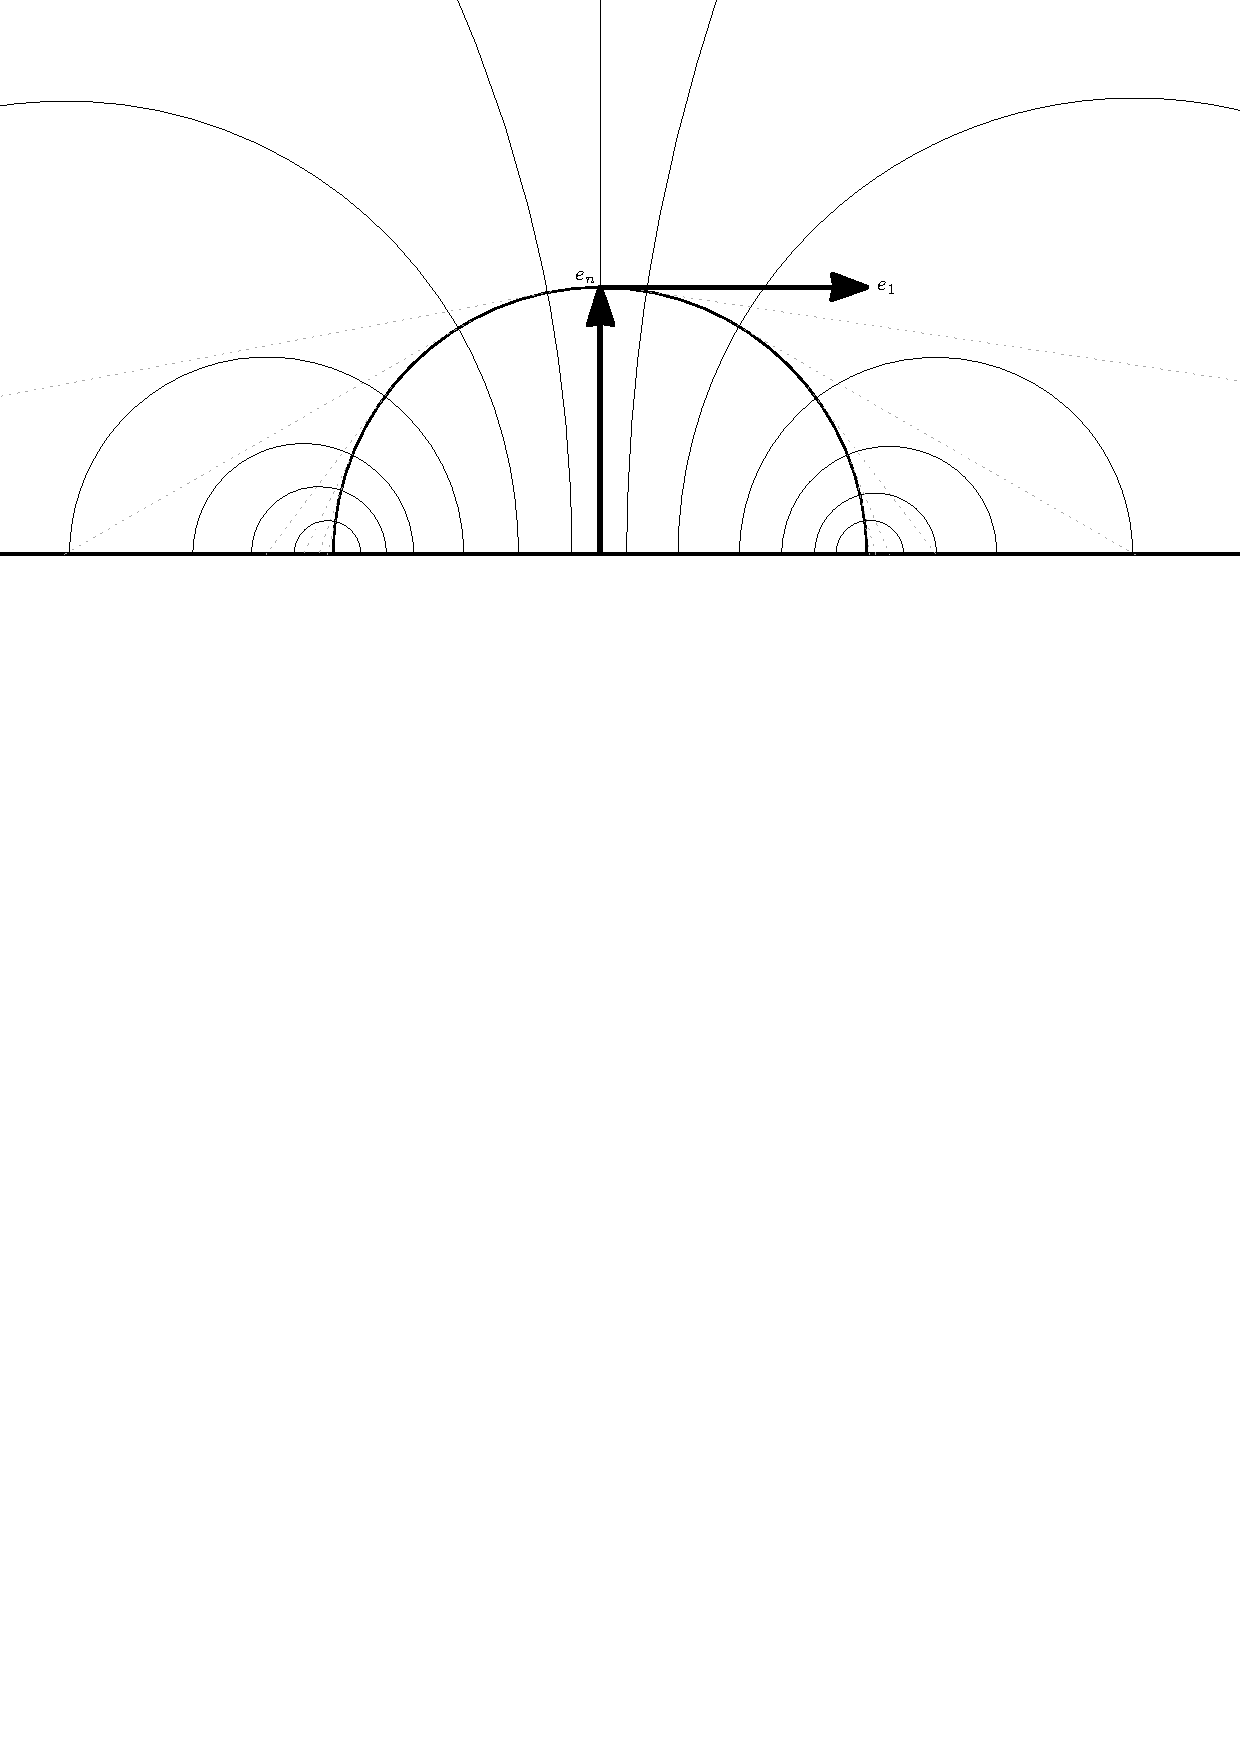
\includegraphics[width=\textwidth]{figures/5b_moving_planes_hyperbolic}
	\caption{The moving hyperplanes in $\mathbb{H}^n$ when the point we chose is $e_n$ and the direction is $e_1$, projected onto the plane spanned by these two vectors. The centres of the hemispheres are the intersection of the $x_n=0$ plane with the line spanned by the tangent vector.}
	\label{moving hyperplanes hyperbolic}
\end{figure}

\begin{oss}\label{inequality1}
	\em Another choice of direction on the hyperbolic plane allows one to write an explicit formula for the reflection about each hyperplanes, which may be more enlightening than the construction above on another important matter. One can repeat the construction, taking the point $e_n$ and direction $e_n$. The geodesic is then the vertical $x_n$ axis and the totally geodesic hyperplanes are therefore the euclidean spheres centred at the origin. Assume without loss of generality that curvature is $\pm 1$, and take the sphere of radius $r$. We claim that the reflection about the sphere of radius $r$ is the spherical inversion about the sphere. We remind the reader that a spherical inversion about a sphere of centre $O$ is a transformation mapping a point $P$ to the point $P'$ on the (euclidean) line through $O$ and $P$ such that $\overline{OP}\cdot \overline{OP'} = r^2$. Therefore the point $(\underline{0}, a)$ on the geodesic is mapped to $(\underline{0}, \frac{r^2}{a})$ by the inversion. Computing the geodesic distance of these two points to  $(\underline{0}, r)$:
	\begin{align*}
		&\int_{r}^{a} \frac{1}{x} dx = \left[\ln{x} \right]_{r}^{a} = \ln{a} - \ln{r} \\
		&\int_{\frac{r^2}{a}}^{r} \frac{1}{x} dx = \left[\ln{x} \right]_{\frac{r^2}{a}}^{r} = \ln{r} - 2 \ln{r} + \ln{a} - \ln{ r} = \ln{a} - \ln{r}
	\end{align*}
	we see that the points are the equidistant from $(\underline{0}, r)$ and therefore the corresponding spheres/hyperplanes have to map to each other. On the other hand, it is an inversion, and inversions are orientation-reversing isometries in hyperbolic space. Please note however that, if we consider $I_r(P)$, for a fixed a point $P\in \mathbb{H}^n$, and let $r$ vary, it does not move along a geodesic unless it is on the geodesic generating the motion. Therefore, as the geodesic is the shortest path, taking $r$ to be varying between $R_0$ and $R_1$
	\begin{align*}
		\mathrm{dist}(I_{R_0}(P), I_{R_1}(P)) \leq \mathrm{length} (I_r(P))
	\end{align*}
	in general, with a strict inequality unless $P$ is on the vertical geodesic. This is unlike the situation on the plane, where equality holds everywhere. 
	The hyperplanes in the euclidean case are equidistant at all points from one another: this cannot be achieved in a curved setting. 
\end{oss}
\begin{oss}\label{inequality2}\em 
	The inequality
	\begin{align}
		\mathrm{dist}(I_{R_0}(P), I_{R_1}(P)) \leq \mathrm{length} (I_r(P))
	\end{align}
	where $I_\cdot(P): t \mapsto (P,t)$ is also the path formed by points of the same space coordinate on the hyperplanes, holds also on $S^n$, because said paths are not geodesics in this case either. 
\end{oss}

\section{The Moving Planes Method}
\label{method moving planes}

The Moving Planes Method is a technique that can be used to prove radial symmetry of certain solutions to some differential equations.  The method was originally introduced by Alexandrov to characterize the sphere as the only hypersurfaces with constant curvature (see for example \cite{alexandrovexample}), and then used by Serrin on elliptic PDEs (see \cite{serrin1971}) and Gidas-Ni-Nirenberg (see \cite{GidasNirenberg}). 

To provide some justification and context to the next chapters, we here describe the method in $\mathbb{M}^{n+1}_+$.  

Let $X:M^n\rightarrow \mathbb{M}^{n+1}_+$ be a hypersurface in a constant curvature ambient space. If the ambient space is a sphere, $X$ must be contained in a hemisphere to avoid issues with multiple self-intersections. Assume also that $X=\partial\Omega$ for a bounded domain $\Omega$ in $\mathbb{M}^{n+1}_+$. 
\begin{itemize}	
	\item As a first step, choose a point a point $O \in \mathbb{M}^n$. As $\mathbb{M}^n$ is a homogeneous space, so the construction does not depend on the choice we make. Without loss of generality, we choose the origin in $\R^n$, $e_n$ in $\mathbb{H}^n$ and the north pole in $S^n$. 
	\item Choose any direction in $v\in T_O\mathbb{M}^n$ and consider the geodesic $\gamma_v: I \rightarrow \mathbb{M}^n$ satisfying $\gamma_v (0) = O$ and $\dot{\gamma_v} (0) = v$. Assume that $\gamma$ is parametrised by arc-length. Here $I=\R$ if $\mathbb{M}^n_+$ is flat or hyperbolic, and  $I=(-\frac{\pi}{2}, \frac{\pi}{2})$ if $\mathbb{M}^n_+$ is a hemisphere.
	\item Consider the hyperplanes $\pi_{v, s}$ passing through $\gamma_v(s)$ and orthogonal to  $\dot{\gamma_v}(s)$.
\end{itemize}
The method consists of reflecting the part of $X$ ``below" the hyperplane into the top part, and using properties of both copies of the hypersurface together to prove some statement about the non-reflected hypersurface. 

To make this more precise, we can define: 
\begin{align*}
	X_{v, s} = \left\{p \in X \;|\; p\in \pi_{v, t} \; \mathrm{ for \; some }\; t < s\right\}
\end{align*}
We will use the notation $X_{v, s}^\pi$ to indicate the reflection of $X_{v, s}$ about $\pi_{v, s}$. 

\begin{figure}
	\centering
	\includegraphics[width=\textwidth]{"figures/6_method moving planes"}
	\caption{The method of the moving planes in $\R^2$. In the figure, the ``plane" is centred for easier pagination, but the hypersurface is fixed and the plane varies. The third figure shows the critical time $m_v$ when the hypersurface and its reflection touch internally.}
\end{figure}

Finally, we define: 
\begin{align*}
m_v &= \sup\left\{s \in I \;|\; X_{v, s}^\pi \subset \Omega \; \mathrm{ for \; every }\; t < s \right\}\\
 &= \sup\left\{s \in I \;|\; X \cap X_{v, s}^\pi =\emptyset \; \mathrm{ for \; every }\; t < s \right\}
\end{align*}
the last time at which the hypersurface and its reflection do not touch internally. Please note that at $m_v$ the two surfaces are tangent at some point, which can be either in the interior of X, or on the boundary. The hyperplane $\pi_{v, m_v}$ is the critical hyperplane. 


\section{The Alexandrov soap-bubble theorem}

To give some justification to the method we described, we will outline the proof an important result that uses this method, the so-called Alexandrov soap bubble theorem. This section will gloss over some technical matters which can be made more precise with some effort. For more details, see \cite{italiani}. 
\begin{comment}
	{\vspace{10pt}\LARGE \bf [DISTANCE SPHERES]}
\end{comment}
\begin{theorem}
	The only $C^2$-regular connected hypersurfaces embedded in $\mathbb{M}^{n+1}_+$ and such that the mean curvature is constant are the distance spheres.\label{Alexandrov theorem} 
\end{theorem}
In \cite{italiani} this theorem is proved more generally: let $H_X$ be a $C^2$ function of the ordered principal curvatures $H_X=f(\kappa_1, \dots, \kappa_n)$, and
\begin{align*}
	f:\{(x_1, \dots, x_n)\in \R^n \;|\;x_1\leq x_2\leq \dots \leq x_n \}\rightarrow \R
\end{align*}
is such that
\begin{align*}
	f(x)>0 \;\mathrm{if \;} x_i>0 \; \mathrm{for \; every \;} i=1, \dots, n
\end{align*}

and it is concave on the component of $\{x\in \R^n \;|\; f(x)>0\}$ containing $\{x\in \R^n \;|\;  x_i>0 \}$. Then the following more general theorem holds: 

\begin{theorem}
	The only $C^2$-regular connected hypersurfaces embedded in $\mathbb{M}^{n+1}_+$ and such that $H_X$ is constant are the distance spheres. 
\end{theorem}

The following proposition holds:

\begin{proposition}
	\label{proposition symmetry conclusion}	Let $X=\partial\Omega$ be a $C^2$-regular, connected, closed hypersurface embedded in $\mathbb{M}^{n+1}_+$, where $\Omega$ is a bounded domain. Assume that for every geodesic $\gamma:\R\rightarrow \mathbb{M}^{n+1}$ there exists a hyperplane orthogonal to $\gamma$ such that $X$ is symmetric about $\pi$. Then $X$ is a distance sphere about its centre of mass $O$, i.e. the unique minimum of 
	\begin{align*}
		P_\Omega(x)=\int_\Omega d(x, a)^2 da
	\end{align*}
\end{proposition}

Its proof is in \cite{italiani} and is omitted here. We now move on to the proof of Theorem \ref{Alexandrov theorem}:
\begin{skproof}
	Assume that $X$ is a manifold with constant mean curvature. 
	We want to show that, for any point $O$ and for every direction $v\in T_O\mathbb{M}^{n+1}$, $X$ is symmetric about a plane perpendicular to the geodesic $\exp_O(tv)$. We put ourselves in the hypothesis of the method of the moving planes described in section \ref{method moving planes}. At $m_v$, $X \cap X_{v, m_v}^\pi$ is non-empty by definition of $m_v$ and therefore it is closed in $X_{v, m_v}^\pi$. We want to show that  $X \cap X_{v, m_v}^\pi$ is an open set in $X_{v, m_v}^\pi$. 
	
	Let $p\in X\cap X_{v, m_v}^\pi$. As the two manifolds are tangent
	\begin{align*}
		T_p X=T_p X_{v, m_v}^\pi.
	\end{align*} By Theorem \ref{localgraphcorollary}, we can represent both manifold as the Euclidean graph of two functions $C^2$ functions $u$ and $\tilde{u}$ defined in a neighbourhood of $p$ inside the tangent space. Consider now the differential equation: 
	\begin{align*}
		K(u(x))=K(\tilde{u}(x))=\;\mathrm{constant} 
	\end{align*}
	where $K$ is the mean-curvature operator. As $X$ is a manifold with constant mean curvature, it holds everywhere. 
	Looking at equation (\ref{Weingarten1}), we see that, given that the principal curvature are a function of the $h_{ij}$, the operator $K$ is an elliptic operator. Reasoning exactly like we did in section \ref{non linear pde parabolic section} for parabolic differential equations, we see that $u-\tilde{u}$ is the solution of a linear elliptic differential equation of the form $L (u-\tilde{u})=0$, with $u(p)=\tilde{u}(p)=0$. 
	
	Without loss of generality, we can assume that, in the neighbourhood where we defined $u$ and $\tilde{u}$, $u-\tilde{u}\geq 0$. 
	
	If $p$ is an interior point in $X_{v, m_v}^\pi$, we can then apply the maximum principle for elliptic equations  (see \cite{Evans} and \cite{protterweinberger}) and obtain that  $u=\tilde{u}$ in the neighbourhood. 
	
	Otherwise, if $p\in\pi_{v,s}$, $\nabla u (p)=\nabla \tilde{u} (p)=0$ and one can apply Hopf's boundary point lemma for elliptic equations (see \cite{Evans} and \cite{protterweinberger}) to conclude again that $u=\tilde{u}$ in the neighbourhood.
	
	Therefore, the whole neighbourhood is in $X\cap X_{v, m_v}^\pi$, hence the intersection is open, as every point $p$ is contained in an open ball. This proves that $X$ is symmetric about $\pi_{v, m_v}$. The theorem is then consequence of Proposition \ref{proposition symmetry conclusion}
\end{skproof}

\begin{oss}
	\em To prove the theorem in the aforementioned more general setting, one would need to only prove that the differential equation $H_X(u(x))= \mathrm{constant}$ is an elliptic equation. Its ellipticity is a standard result in Geometric Analysis, and can be found in many other works. It is also equivalent to equation (\ref{evolutioneq}) being parabolic (see section \ref{parabolic}).
\end{oss}

% !TeX spellcheck = en_GB
\chapter{The Chow-Gulliver Critical Planes Result}

The main result we want to establish in this chapter is theorem \ref{chow gulliver}, a result about critical hyperplanes when applying the method of the moving planes to solution of a large class of non-linear parabolic partial differential equations, and whose proof is somewhat similar to Theorem \ref{Alexandrov theorem}. 

We will first describe the differential equations we are analysing, then prove that they are parabolic, then prove the theorem. 

\section{Class of Equations we analyze}

We consider manifolds $M^n$ embedded in $\R^{n+1}$, i.e. there is an embedding $X_0 : M^n \rightarrow \R^{n+1}$ parametrizing the hypersurface $X_0(M^n)$. 

Let $F:\{(\kappa_1, \dots , \kappa_n)\in \R^n\vert \kappa_1\leq \dots \leq \kappa_n\}\rightarrow \R$ be a $C^1$ function satisfying:

\begin{equation}
	\frac{\partial F}{\partial \kappa_i} > 0 \mathrm{\; for \; all } \; i=1,\dots, n \label{parabolicità}
\end{equation}
and consider the evolution equation 
\begin{align}
	\begin{dcases}
		\frac{\partial X_t}{\partial t} = - F(\kappa_1(x), \dots , \kappa_n(x)) \nu\\
		X(0)= X_0
	\end{dcases} \label{evolutioneq}
\end{align}
where $\nu$ is the outward normal to $X_t(M^n)$ at the point $X_t(x)$ and $\kappa_1\leq \dots \leq \kappa_n$ are the principal curvatures at $X_t(x)$. 


\section{Parabolicity of the differential equation (\ref{evolutioneq})}\label{parabolic}


The condition (\ref{parabolicità}) will  guarantee that equation (\ref{evolutioneq}) is a parabolic equation. This may be confusing, as (\ref{evolutioneq}) does not make it obvious how to apply definition \ref{nonlinearpde}. 

In order to classify a non-linear partial differential equation one has to understand how it behaves ``close to a solution" in the solutions space. We want to prove that very close to any solution, ``moving in any direction", the change in the equation is always a parabolic PDE. This will then tell us that our equation is parabolic, and that the theorems that apply to solutions of parabolic partial differential equations apply to our equation as well. To do so, we are going to ``linearise" the differential equation about a solution.

Like in \cite{huisken}, as $F$ is a symmetric function in the principal curvatures, we may interchangeably take $F$ to be a function of the Weingarten map tensor or of the second fundamental form, and thus we get:

\begin{align*}
	\frac{\partial X_t}{\partial t} &= - F(h_{ij}(X_t)) \nu
\end{align*}

To understand the behaviour close to a solution, we can substitute in our equation $X_t$ with a $X_t+\varepsilon u_t$ to get:

\begin{align}
	\frac{\partial X_t}{\partial t} + \varepsilon\frac{\partial u_t}{\partial t}  &= - F(h_{ij}(X_t+\varepsilon u_t)) \nu_{(X_t+\varepsilon u_t)}\label{linearizingevolutioneq}
\end{align}
where we mean that  $\nu_{(X_t+\varepsilon u_t)}$ is the normal to the perturbed immersion. 
We are interested in the behaviour of this equation for a small $\varepsilon$. This equation when taking the limit for $\varepsilon \rightarrow 0$ is the so-called linearisation of the PDE; we want this PDE to be a parabolic equation to apply our results.

We can use the Weingarten equation (\ref{Weingarten1}) to write the RHS explicitly:

\begin{align*}
	h_{ij}(X_t& + \varepsilon u_t )=-\left\langle v, \nu_{(X_t+\varepsilon u_t)}\right\rangle\; \mathrm{where}\\
	v^\alpha=&\; \frac{\partial^2 X_t^\alpha}{\partial x^i \partial x^j} - \Gamma^k_{ij}\frac{\partial X_t^\alpha}{\partial x^k}+\overline{\Gamma}^\alpha_{\beta \delta}\frac{\partial X_t^\beta}{\partial x^i}\frac{\partial X_t^\delta}{\partial x^k} +\\ %epsilon
	&+\varepsilon\left(\frac{\partial^2 u_t^\alpha}{\partial x^i \partial x^j} - \Gamma^k_{ij}\frac{\partial u_t^\alpha}{\partial x^k}+\overline{\Gamma}^\alpha_{\beta \delta}\left(\frac{\partial X_t^\beta}{\partial x^i}\frac{\partial u_t^\delta}{\partial x^k} + \frac{\partial u_t^\beta}{\partial x^i}\frac{\partial X_t^\delta}{\partial x^k}\right)\right)+\\
	%epsilon squared
	&+\varepsilon^2\left(\overline{\Gamma}^\alpha_{\beta \delta}\frac{\partial u_t^\beta}{\partial x^i}\frac{\partial u_t^\delta}{\partial x^k}\right) \\
	v^\alpha=&\; w +\varepsilon\left(\frac{\partial^2 u_t^\alpha}{\partial x^i \partial x^j} + \mathrm{lower \; order \;  terms}\right) + o(\varepsilon)
\end{align*}
where $h_{ij}(X_t)=-\left\langle w, \nu_{X_t}\right\rangle$.

Putting it all together in the first line:
\begin{align*}
	h_{ij}(X_t + \varepsilon u_t ) &=-\left\langle  w +\varepsilon\left(\frac{\partial^2 u_t}{\partial x^i \partial x^j} + \mathrm{lower \; order \;  terms}\right) + o(\varepsilon), \nu_{(X_t+\varepsilon u_t)}\right\rangle\\
	&= \left\langle  w, \nu_{(X_t+\varepsilon u_t)}\right\rangle -\varepsilon\left\langle  \left(\frac{\partial^2 u_t}{\partial x^i \partial x^j} + \mathrm{lower \; order \;  terms}\right), \nu_{(X_t+\varepsilon u_t)}\right\rangle + o(\varepsilon)\\
	&= h_{ij}(X_t) + \left\langle  w, \nu_{(X_t+\varepsilon u_t)}-\nu_{X_t}\right\rangle -\varepsilon H_{ij} + o(\varepsilon)\\
	&= h_{ij}(X_t) -\varepsilon H_{ij} + o(\varepsilon)
\end{align*}
Were on the last step we are using the fact that $\nu_{(X_t+\varepsilon u_t)}-\nu_{X_t} = O(\varepsilon)$, and as this gets smaller the component of w parallel to the difference also is $O(\varepsilon)$, as $w$ is parallel to $\nu_{X_t}$.
We can then expand F in the RHS of the equation (\ref{linearizingevolutioneq}) to the first order, as it is a $C^1$ function: 
\begin{align*}
	\cancel{\frac{\partial X_t}{\partial t}} + \varepsilon\frac{\partial u_t}{\partial t}  &= - \left(\cancel{F(h_{ij}(X_t)) }
	+ \varepsilon \langle DF, H\rangle + o(\varepsilon)\right)\nu_{(X_t+\varepsilon u_t)}\\
	\varepsilon\frac{\partial u_t}{\partial t}  &= \varepsilon\left(
	\frac{\partial F}{\partial h_{i j}} g^{i k}g^{jl}\left\langle \frac{\partial^2 u_t}{\partial x^k \partial x^l},  \nu_{(X_t+\varepsilon u_t)}\right\rangle + \mathrm{lower \; order \;  terms}\right)\nu_{(X_t+\varepsilon u_t)} + o(\varepsilon)\\
	\frac{\partial u_t}{\partial t}  &= 
	\frac{\partial F}{\partial h_{i j}} g^{i k}g^{jl}\left\langle \frac{\partial^2 u_t}{\partial x^k \partial x^l},  \nu_{(X_t+\varepsilon u_t)}\right\rangle \nu_{(X_t+\varepsilon u_t)} + \mathrm{lower \; order \;  terms} + o(1)
\end{align*}
Letting $\varepsilon\rightarrow 0$, we get to: 

%Here, $\delta h_{ij}(u_t)=\frac{h_{ij}(X_t+\varepsilon u_t)-h_{ij}(X_t)}{\varepsilon}=\frac{h_{ij}(\varepsilon u_t)}{\varepsilon}=h_{ij}(u_t)$ by linearity of the definition of the second fundamental form. 
%\begin{align*}
%	\frac{\partial u_t}{\partial t}  &=  DF(h_{ij}(u_t)) \nu\\
%	\frac{\partial u_t}{\partial t} &= \frac{\partial F}{\partial h_{i j}} g^{i k}g^{jl}h_{k l}(u_t) \nu
%\end{align*}
%
%Using the Weingarten Equations this becomes, implying Einstein's summation convention: 
\begin{align*}
	\frac{\partial u_t}{\partial t} &= \frac{\partial F}{\partial h_{i j}} g^{i k}g^{jl}\left\langle \frac{\partial^2 u_t}{\partial x_k\partial x_l} , \nu \right\rangle \nu+ \mathrm{lower \ order \ terms}
\end{align*}
For the second order term to be positive definite, then, 
\begin{align*}
	\left(\frac{\partial F}{\partial h_{i j}} \right)_{i, j}
\end{align*}
must be positive definite. Or equivalently, as the principal curvatures are the eigenvalues of the matrix $(h_{i j})_{i, j}$,
\begin{align*}
	\frac{\partial F}{\partial \kappa_{i}} > 0
\end{align*}
A more general approach proving that the differential equation is parabolic can be found in \cite{Gerhardt Curvature}. 
\begin{comment}
	{\em Looking more closely at what we are doing, one can prove that it is equivalent to follow this linearisation procedure or to take the derivatives of $F$ with respect to the second order terms.}
\end{comment}

\begin{oss}
	{\em While in this chapter we are using the standard metric of $\R^n$, the proof above is valid using any other metric.}
\end{oss}
\begin{comment}
	contenuto...
	If one considers the F which are linear in the $\kappa_{i}$, this yields:  
	
	\begin{align*}
		\frac{\partial Y_t}{\partial t} &= \left(\frac{\partial F}{\partial\kappa_{i}} \kappa_{i} \right)\nu\\
		\frac{\partial Y_t}{\partial t} &= \frac{\partial F}{\partial\kappa_{i}} o^{ik} h_{kl}o^{li}\,\nu \\ 
		\frac{\partial Y_t}{\partial t} &= \frac{\partial F}{\partial\kappa_{i}}   o^{ik}o^{li}\left\langle \frac{\partial^2 Y_t}{\partial x_k\partial x_l} , \nu \right\rangle \,\nu + \text{lower order terms}
	\end{align*}
	implying summation convention, for an appropriate orthogonal matrix $o_{li}$ that makes $h_{ij}$ diagonal, which makes the equation parabolic if $\frac{\partial F}{\partial \kappa_i}$ is positive. 
	
	{\vspace{10pt}\LARGE \bf [NEED HELP WITH PARABOLICITY!]}
	
	In \cite{huisken}, the paper considers F as a function of the second fundamental form $h_{ij}$, as the principal curvatures are themselves function of it. The following is then said, speaking about "linearisation", while also citing the Weingarten equations:
	\begin{align*}
		\frac{\partial Y_t}{\partial t} &= \frac{\partial F}{\partial h_{i j}} g^{i k}g^{jl}h_{k l} \nu+ \mathrm{lower \ order \ terms}\\
		\frac{\partial Y_t}{\partial t} &= \frac{\partial F}{\partial h_{i j}} g^{i k}g^{jl}\left\langle \frac{\partial^2 Y_t}{\partial x_k\partial x_l} , \nu \right\rangle \nu+ \mathrm{lower \ order \ terms}
	\end{align*}
	Which I did not understand the implication of (especially with respect to maximum principle - there is probably something I am missing due to non-linearity of the equation). 
	
	\begin{theorem}[Parabolicity of the differential equation (\ref{evolutioneq})]
		da scrivere\label{graphparabolic}
	\end{theorem}
	
	Il conto probabilmente è quello in \cite{hamilton}, pagina 262. Info sul nostro caso sono in \cite{huisken}, pagina 50. 
	
	{\vspace{10pt}\LARGE \bf [NEED HELP!]}
	
\end{comment}

\section{An existence result}
In \cite{huisken} one finds the following comforting existence result for the class of equations we are analysing under very broad hypothesis. The same paper also includes a proof of the result with some more restrictive hypotheses. A complete proof is quite more involved. We will not use it, nor prove it, but it is included here for completeness and peace of mind: 

\begin{theorem}[Short term existence of a solution for (\ref{evolutioneq})]
	Suppose $X_0 : M^n \rightarrow \R^{n+1}$ is a smooth, closed hypersurface in $\R^{n+1}$, such that (\ref{parabolicità}) holds at all points in $X_0$, i.e. for all the values of the principal curvatures $\kappa_{i}$ realized at some point on $X_0$. Then, (\ref{evolutioneq}) has a smooth solution, at least on some short time interval $[0, T)$, $T > 0$.  \label{existence}
\end{theorem}

A much more extended analysis of the problem of the existence of solution to the equation can be found in \cite{Gerhardt Curvature}. 


\section{Local representation as a graph of a solution of (\ref{evolutioneq})}
\label{representation as graph}
As a first step, from the Corollary \ref{localgraphcorollary}, we can establish the following:

\begin{theorem}[Local representation as a graph of a solution of (\ref{evolutioneq})]
	Let $X^n$ be a submanifold $X^n\subset\R^{n+1}$ and let $F:X^n\times(0, T)\rightarrow \R^{n+1}$ be a solution of (\ref{evolutioneq}). Also let $t\in(0, T)$ and $x\in F(X^n, t)$.
	Then there exists a neighbourhood of $(x, t)$, $U\subset F(X^n\times(0, T))$, and a smooth function $f: T_{x} F(X^n, t)\times(0, T)\rightarrow \R$ such that any $(x_0, t_0)\in U$ can be expressed as 
	\begin{align*}
		x_0= p +f(p, t_0) \nu 
	\end{align*}
	where $\nu$ is a vector normal to $T_{x} F(X^n, t)$, for an appropriate point $p\in T_x F(X^n, t)$. \label{localgraph}
\end{theorem}
\begin{comment}
	{\vspace{10pt}\LARGE \bf [NON FUNZIONA! Difficile (impossibile?)dimostrare che è smooth]}
	With a reasoning similar to \ref{localgraphclassic} and \ref{localgraphcorollary} one can prove that given any plane, we can represent locally a manifold $M\subset\R^{n+1}$ at $x\in M$ as a graph on that plane, i.e. as $x_0= p + f(p) \nu$ for $\nu$ the vector orthogonal to the plane, as long as $\nu\notin T_xM$. 
	The function which associates to $t\in [0,T)$ the unit vector orthogonal to $T_{F(x, t)}F(X, t)$ is continuous, as $F$ is smooth and the vector can be computed from the derivatives of the local maps of the manifold. Thus we can find a neighbourhood $(a,b)$ of $ t_0$ such that for $t \in (a,b)$ the normal vector is not in $T_x F(X^n, t)$. In $(a,b)$ we can represent $F(X)
\end{comment}


\begin{proof}
	We can consider the image of $F:X^n\times(0, T)\rightarrow \R^{n+1}$ as a manifold in $\R^{n+2}$ by considering $G:=(F(x, t), t)$. Moreover $\frac{\partial G_t}{\partial e_j}\equiv 0$ for all possible vectors of the canonical basis of $\R^{n+1}\times \R$ except for the one corresponding to the time coordinate, where it is $1$. Also, $\frac{\partial G_i}{\partial e_j}\equiv \frac{\partial F_i}{\partial e_j}$ and the first $n$ coordinates of  $\frac{\partial G}{\partial t}$ form a vector normal to $T_x X^n$ by (\ref{evolutioneq}).  Thus, the tangent space of $\mathrm{Im}(G)$ is $T_x X^n \times \{0\}\oplus  \mathrm{span}\langle (\nu, 1)\rangle$ and we can apply corollary  \ref{localgraphcorollary} to $\mathrm{Im}(G)$ to get a function $\tilde{f}$ such that 
	\begin{align*}
		(x_0, t)= \left[(p, 0) +  (s\nu, s)\right] + \tilde{f}(p, s)(\nu, -\Vert \nu\Vert)
	\end{align*}
	as $(\nu, -\Vert \nu\Vert)$ is the vector orthogonal to  $T_x X^n \times \{0\}\oplus  \mathrm{span}\langle (\nu, 1)\rangle$. Let $\sigma_p:I\subset\R\rightarrow\R$ be the function that associates to $t$ the appropriate $s$ in the expression above.  Projecting to the first $n+1$ coordinates and calling $f(p, t)=\sigma_p(t)+\tilde{f}(p, \sigma_p(t))$ one gets:
	\begin{align*}
		x_0= p + f(p, t)\nu 
	\end{align*}
	which is our thesis, as long as $\sigma_p(t)$ is smooth. This is indeed the case, as the graph function $\Gamma_f:x\mapsto(x, f(x))$ is smooth for any smooth function $f$ and has a smooth inverse (and thus, the inverse $(x_0, t)\mapsto ((p, 0) +  (s\nu, s))$ is smooth).
\end{proof}
One can show through direct calculation (see \cite{mantegazza}, Exercise 1.1.2) that, if an immersed hypersurface $\phi : M\rightarrow \R^{n+1}$ is locally the graph of a function $f:\R^n \rightarrow \R$ (i.e., locally, $(x, f(x))=\phi$), then: 
\begin{align*}
	g_{ij}&=\delta_{ij}+ \frac{\partial f}{\partial x_i} \frac{\partial f}{\partial x_j}\\
	\nu&= -\frac{(\nabla f, -1)}{\sqrt{1+|\nabla f|^2}}\\
	h_{ij}&= -\frac{H_{ij}}{\sqrt{1+|\nabla f|^2}}
\end{align*}
Where the matrix $(H_{ij})_{ij}$ is the hessian of $f$. Thus, if one considers the principal curvatures, they are closely related to the eigenvalues of the hessian of $f$. 




\section{The Moving Planes Method and the Chow result}

We will now present the Chow-Gulliver result, presented more or less as in paragraph 2 in \cite{Chow}.
Suppose that we have a hypersurface embedded in $\R^{n+1}$ evolving according to equation (\ref{evolutioneq}). For a fixed time $t$, we can apply the method of the moving planes as described in section \ref{method moving planes}: we can take parallel hyperplanes $\pi_{v,s}$ orthogonal to $v$ intersecting $X$, and consider the reflection  $X_{v,s}^\pi$. There will be a hyperplane $\pi_{v,m_v}$ where $X$ and $X_{v,s}^\pi$ are tangent. As the hypersurface evolves, we may wonder how this critical threshold changes over time. If it behaves in a predictable way, we can hope to use the technique on the evolving manifold, otherwise, it may be hopeless if the critical plane moves back and forth multiple times. In the next section, we are going to prove a result in this general direction, to show a form of "regularity" in this sense. First, however, we need to introduce a marginally stricter definition for the concept of "reflecting inside itself". 



Let $\pi$ be a hyperplane in $\R^{n+1}$. We may assume $\pi$ orthogonal to a unit vector $v\in\R^{n+1}$, i.e. $\langle x, v\rangle= C$ for all $x\in \pi$ for some constant $C$. In our notation for the method of moving planes, assuming we pick the origin as a starting point, this means that $\pi = \pi_{v, C}$. 

Then, $\R^{n+1}$ is divided by $\pi$ into two half-spaces, which we will name 
\begin{align*}
H^+(\pi)&=\{x \in \R^{n+1} : \langle x, v\rangle > C\}= \bigcup_{s>C} \pi_{v, s} \;\;\mathrm{and}\\
H^-(\pi)&=\{x \in \R^{n+1} : \langle x, v\rangle < C\}= \bigcup_{s<C} \pi_{v, s}.
\end{align*} 

\begin{defin}
	We say {\em we can reflect $X: M^n\rightarrow \R^{n+1}$ strictly with respect to $\pi$} if both:
	\begin{itemize}
		\item $X^\pi\cap H^-(\pi)\subset \mathrm{int}(X)\cap H^-(\pi)$ where $X^\pi$ is the reflection of $X$ about $\pi$ and $\mathrm{int}(X)$ is the region inside $X$.
		\item $V\notin T_xM$ for all $x\in M^n \cap\pi$
	\end{itemize} \label{strict-reflection-definition}
\end{defin}


\begin{figure}
	\centering
	\includegraphics[width=\textwidth]{"figures/7_reflects_strictly"}
	\caption{Example: We can reflect $X: M^n\rightarrow \R^{n+1}$ strictly with respect to $\pi$}
\end{figure}

\begin{figure}
	\centering
	\includegraphics[width=\textwidth]{"figures/8_interior_contact"}
	\caption{Example: We cannot reflect $X: M^n\rightarrow \R^{n+1}$ strictly with respect to $\pi$, because there is an interior contact}
\end{figure}
\begin{figure}
\centering
\includegraphics[width=\textwidth]{"figures/9_boundary_contact"}
\caption{Example: We cannot reflect $X: M^n\rightarrow \R^{n+1}$ strictly with respect to $\pi$, because the tangent spaces coincide at a point about which we are reflecting}
\end{figure}

This fundamentally means that the reflection of one of the halves of $X$ on the other side of $\pi$ is contained in the region inside $M^n$ and the tangent spaces of $X$ and of the half-reflection do not form a ninety degree angle with $\pi$, at all points on $\pi\cap X$. As the two tangent spaces are one the reflection of the other, this means that they do not coincide.   
\begin{defin}
	We say {\em we can reflect $X: M^n\rightarrow \R^{n+1}$ strictly up to $(\pi,v)$} if we can reflect $M^n$ strictly with respect to $\pi_{v, s}$ for all hyperplanes $\pi_{v, s}$ such that $s<C$.  
\end{defin}

The key idea of the main result in the next section is as follows: suppose we have an embedded smooth hypersurface $X$ evolving according to (\ref{evolutioneq}) and a fixed hyperplane $\pi$, intersecting $X$. Suppose that, at some time $t$, $X$ and  $X_\pi$ touch outside of $\pi$. We can consider $X$ and  $X_\pi$ as local graphs over the same hyperplane $\pi$, and we can show that these function evolve according to the same differential equation. Using the strong maximum principle and the Hopf boundary point lemma, then, one can conclude that the two functions coincide, and have been coinciding up until that point. We can then conclude that if  $X$ and  $X_\pi$ only touch in $X\cap\pi$ at the beginning of the evolution, then they will never touch elsewhere.  


\section{The Chow-Gulliver result}

The main theorem is the following: 

\begin{theorem}[Chow-Gulliver]\label{chow gulliver}
	Let $X:M^n\times [0,T) \rightarrow \R^{n+1}$ be a $C^2$ solution to equation (\ref{evolutioneq}). Then, if we can reflect $X(M^n, 0)=X_0$ strictly with respect to $\pi$, then for all $t\in [0,T)$ we can reflect $X(M^n, t)=X_t$ strictly with respect to $\pi$. 
\end{theorem}

\begin{proof}
	By contradiction, suppose that there is a time $t$ such that the thesis is false, and that it is the smallest such $t$. Then, for all $\tau \in [0,t)$, $X_{\tau,\pi}\cap H^-(\pi)\subset \mathrm{int}(X_{\tau})\cap H^-(\pi)$; the unit vector orthogonal to $\pi$, $V$, is such that $V\notin T_xX_\tau$ for all $x\in X_\tau\cap \pi$ and $\tau \in [0,t)$; and either of the conditions fails at $t$, i.e. either: 
	\begin{itemize}
		\item[(i)] $X_{t,\pi}\cap H^-(\pi)\cap X_{t}\neq \emptyset$
		\item[(ii)] $V\in T_xX_t$  for some $x\in\pi$. 
	\end{itemize} 
	
	(i) Suppose the first case is true. Then, there exists $x_0 \in X_{t,\pi}\cap H^-(\pi)\cap X_{t}$ such that at $x_0$ the two manifolds are tangent. \\
	We can take a neighbourhood of $(x_0, t)\in X_{t}\times \R$ such that  both $X_{t,\pi}$ and $X_{t}$ are graphs over $T_{x_0}X_{t}$ by \ref{localgraph}. \\
	We can explicitly write the functions $f:U\times (t-\varepsilon, t+\varepsilon)\rightarrow X_t$, where $U\subset T_{x_0}X_{t}$, and the corresponding $f_\pi$ for $X_{t,\pi}$. 
	We can also write 
	\begin{align*}
		f \; : \; (x, t) &\mapsto x+\tilde{f}(x, t)\nu \\
		f_\pi \; : \; (x, t) &\mapsto x+\tilde{f}_\pi(x, t)\nu 
	\end{align*}
	for appropriate functions $\tilde{f}:U\times (t-\varepsilon, t+\varepsilon)\rightarrow \R$ and $\tilde{f}_\pi:U\times (t-\varepsilon, t+\varepsilon)\rightarrow \R$, where $\nu$ is a fixed unit vector normal to $T_{x_0}X_{t}$.  $\tilde{f}$ and $\tilde{f_\pi}$ are solutions to the same second order PDE, which is parabolic by what was discussed in paragraph \ref{parabolic}, hence we can apply Proposition \ref{firstapplication} to conclude that $\tilde{f}\equiv\tilde{f_\pi}$, and thus $X_{t,\pi}$ and $X_{t}$ coincide in a neighbourhood of $(x, t)$, a contradiction as we assumed that $t$ is the first $t$ where the flows touch.
	
	(ii) Suppose instead that $V\in T_xX_t$  for some $t\in [0, t)$ and some $x\in X_t\cap \pi$. Then $T_xX_t= T_xX_{t, \pi}$ and in a neighbourhood of $(x, t)$ both $X_t$ and $X_{t, \pi}$ are graphs of two smooth functions over $T_xX_t$ by \ref{localgraph}, i.e. again
	\begin{align*}
		f \; : \; (x, t) &\mapsto x+\tilde{f}(x, t)\nu \\
		f_\pi \; : \; (x, t) &\mapsto x+\tilde{f}_\pi(x, t)\nu 
	\end{align*} 
	Moreover, in $\overline{H^-(\pi)}$, $f_\pi\geq f$, because $M^n_\pi\cap H^-(\pi)\subset \mathrm{int}(M^n)\cap H^-(\pi)$. Finally, $f(x, t)=f_\pi (x, t)$, hence $f_\pi-f (x, t)=0$, and thus  $(x, t)$ is a minimum point on the boundary for $f_\pi-f$. Also, we must have
	\begin{align*}
		\frac{\partial f}{\partial V}(x,t)=\frac{\partial f_\pi}{\partial V}(x,t)
	\end{align*}
	because the graphs are both tangent to $T_xX_t$, and $V$ here is the outward pointing normal to the boundary by definition of the reflection. Thus, 
	\begin{align*}
		\frac{\partial (f- f_\pi)}{\partial V}(x,t)=0
	\end{align*}
	But we must have 
	\begin{align*}
		\frac{\partial (f- f_\pi)}{\partial V}(x,t)>0
	\end{align*}
	at a minimum on the boundary by Proposition \ref{secondapplication}, a contradiction.  
\end{proof}


\section{Some corollaries of the result} 
In this section we collect a number of corollaries to the main result above. This first one is an immediate consequence of the main result:
\begin{cor}
	Let $X:M^n\times [0,T) \rightarrow \R^{n+1}$ be a $C^2$ embedded solution to equation (\ref{evolutioneq}). Then, if we can reflect $X_0$ strictly up to $(\pi_{v,C},v)$, then for all $t\in [0,T)$ $v\notin T_xX_t$ for all $x\in X_t\cap\overline{H^+(\pi)}$. In particular,  $ X_t\cap\overline{H^+(\pi)}$ is a graph over $\pi$ for all $t\in [0,T)$.\label{graph}
\end{cor}




Another immediate consequence of Theorem \ref{chow gulliver} is the following:
\begin{cor}
	Let $X:M^n\times [0,T) \rightarrow \R^{n+1}$ be a $C^2$ solution to equation (\ref{evolutioneq}). Then, if we can reflect $X_0$ strictly up to $(\pi_{v,C},v)$, then for all $t\in [0,T)$ we can reflect $X(M, t)$ strictly up to $(\pi_{v,C},v)$.  
\end{cor}
\begin{proof}
	The hypothesis of the theorem are true for each $\pi_K$ in the definition, thus we can reflect strictly with respect to each $\pi_K$ for all $t\in[0,T)$, and thus we can reflect $X(M, t)$ strictly up to $(\pi_{v,C},v)$.
\end{proof}

 Furthermore, it is clear that for every direction $v$ there exists a hyperplane $\Pi$ perpendicular to $v$ such that we can reflect $X_0$ up to $(\Pi, v)$ and $\Pi$ intersects the interior of $X_0$. To be more precise, for every direction $v$ there exists a hyperplane $\Pi_0^v$ tangent to $X_0$ and such that $X_0\cap H^+(\Pi_0^v)=\emptyset$. Suppose that for every $\varepsilon>0$ we can find a plane $\pi_\varepsilon$ such $H^+(\pi_\varepsilon)\cap B_{R-\varepsilon}(C)=\emptyset$ and we cannot reflect $X_0$ strictly at $\pi_\varepsilon$, where $R$ is such that $X_0 \subset B_R (C)$. We can take the corresponding plane $\Pi_0^\varepsilon$ parallel to $\pi_\varepsilon$ and tangent to $X_0$ at the point $p_\varepsilon$. Taking a sequence $\varepsilon_n \rightarrow 0$ we find a corresponding limited sequence $p_{\varepsilon_n}$ which, by compactness, converges to a point $p\in X_0$. This point $p$ is such that arbitrarily close to it there is a point such that we cannot reflect by more than any chosen $\varepsilon>0$ in the direction of its normal. As we can always represent $X_0$ as the graph of a function in a neighbourhood of $p$, we get a contradiction, because strict reflection in the direction of the normal by at least a fixed uniform amount $\varepsilon$ at each point is always possible locally for any graph of a smooth function. Thus, we obtain the following:
 
\begin{cor}
	Let $X:M^n\times [0,T) \rightarrow \R^{n+1}$ be a $C^2$ embedded solution to equation (\ref{evolutioneq}). There exists $\varepsilon>0$ depending only on $X_0$ such that for all $t\in[0, T)$ we can reflect $X_t$ up to $(\Pi_0^v +\epsilon v, v)$ for every $v \in S^n$. In particular, if $X_0 \subset B_R (C)$, then we can always reflect $X_t$ up to $(\Pi, v)$ whenever $H^+(\Pi)\cap B_{R-\varepsilon}(C)=\emptyset$.\label{reflect a small bit}
\end{cor}
In other words, we can always reflect a little $\varepsilon$ in any direction, uniformly. We can use the fact that we can always reflect about a plane outside a sphere containing $X_0$ to prove the following estimate:




\begin{cor}
	Let $X:M^n\times [0,T) \rightarrow \R^{n+1}$ be a $C^2$ embedded solution to equation (\ref{evolutioneq}). There exists $C>0$ depending only on $X_0$ such that for all $t\in[0, T)$: 
	\begin{align*}
		\max_{x\in X_t} |x| - \min_{x\in X_t} |x| < C
	\end{align*}
\end{cor}
\begin{proof}
	We can reflect $X_0\subset B_R(0)$ up to any plane tangent to  $B_R(0)$, i.e. any plane $\pi_{v, K}$ for any $K\geq R$ and $v$ unit vector, i.e.  $\pi_{v, K}=\{p \in \R^{n+1} : \langle p, v \rangle = K\}$. Let $x_1, x_2\in X_t$ such that $|x_1|=\min_{x\in X_t} |x|$ and  $|x_2|=\max_{x\in X_t} |x|$. Let $v=\frac{x_2-x_1}{\vert x_2-x_1 \vert}$: we can reflect $X_t$ up to $(\pi_{v, R}, v)$ by theorem \ref{chow gulliver}, therefore $\mathrm{dist}(x_2, \pi_{v, R}) < \mathrm{dist}(x_1, \pi_{v, R})$, or in other words:
	\begin{align*}
		 \left\langle x_2, \frac{x_2-x_1}{\vert x_2-x_1 \vert} \right\rangle - R &< 
		 \left\langle x_1, \frac{x_1-x_2}{\vert x_2-x_1 \vert} \right\rangle + R\\
		 \frac{|x_2|^2}{\vert x_2-x_1 \vert} - \cancel{\frac{\left\langle x_2, x_1\right\rangle}{\vert x_2-x_1 \vert}}  - R &< 
		 \frac{\vert x_1\vert^2}{\vert x_2-x_1 \vert} - \cancel{\frac{\left\langle x_2, x_1\right\rangle}{\vert x_2-x_1 \vert}}  + R\\
		 \frac{|x_2|^2 - |x_1|^2}{\vert x_2-x_1 \vert} &< 
		  2R\\
		  |x_2|^2 - |x_1|^2 &< 
		  2R \vert x_2-x_1 \vert \leq 4R |x_2|\\
		  |x_2|^2 &<|x_1|^2 + 4R |x_2|\\
		  |x_2| &< |x_1| \frac{|x_1|}{|x_2|} + 4R < |x_1| + 4R\\
		  |x_2| -|x_1| &<4R
	\end{align*}
\end{proof}


Lastly: 
\begin{cor}
	Let $X:M^n\times [0,T) \rightarrow \R^{n+1}$ be a $C^2$ embedded solution to  equation (\ref{evolutioneq}). Let $s_v:[0,T) \rightarrow I$ be such that 
	\begin{align*}
		s_v(t)= \sup\left\{s \in I \;|\;  \; \mathrm{we \; can \; reflect \;} X_t \mathrm{ \; strictly \; up \; to }\; (\pi_{v, s}, v) \right\}.
	\end{align*}
	Then $s_v(t)$ is a non-decreasing function. Also, if $X_0$ is compact, the limit
	\begin{align*}
		\lim_{t\rightarrow T^-} s_v(t)
	\end{align*}
	exists and is finite.
\end{cor}
\begin{proof}
	When taking $X_t$ as the starting manifold, the hypothesis of the theorem are still true, therefore we can reflect about $\pi_{c, v}$  for all $c<s_v(t)$ at all subsequent times. Thus $s_v(t)$ is non-decreasing. $\lim_{t\rightarrow T^-} s_v(t) = \sup s_v(t)$, therefore the limit exists. Also, if $X_0$ is bounded, there exists $R>0$ such that $X_0\subset B_R(0)$, therefore we can reflect $X_0$ strictly about any hyperplane non intersecting $B_R(0)$, as it does not touch $X_0$, and therefore we can also reflect $X_t$ strictly about the same hyperplanes by theorem \ref{chow gulliver}. At the same time, there exists a hyperplane such that $X_t$ cannot be reflected strictly about it, because there will always be a straight line parallel to $v$ intersecting $X_t$ in multiple points, and we can always consider the hyperplane orthogonal to $v$ passing through their midpoint, about which $X_t$ cannot be reflected strictly, and $s_v(t) \neq +\infty$. Therefore  $s_v(t)\in [-R, R]$, and the limit above is finite. 
\end{proof}


\section{Applying the result to find gradient estimates}

In this section we collect some applications of theorem \ref{chow gulliver} to gradient estimates for the support function and the radial function from \cite{Chow} (a more in-depth definition these two functions can be found in the introduction of \cite{tomography}). Central in what will follow is this corollary providing an estimate for the tangent component of the position vector $x$ of a point on the hypersurface in its own tangent space: 
\begin{cor}
	Let $ X : M^n \times [0, T) \to \mathbb{R}^{n+1} $ be an embedded solution to equation (\ref{evolutioneq}). There exists a constant $ C $, depending only on the initial hypersurface $ X_0 $, such that for all points $ x \in X_t $ and $ t \in [0, T) $, the following inequality holds:
	\begin{align*}
		| x - \langle x \cdot \nu\rangle \nu | \leq C,
	\end{align*}
	where $ \nu $ is the unit normal to $ X_t $ at the point $ x $.
	\label{x projection estimate}
\end{cor}


\begin{proof}: 
	Choose $ C > 0 $ such that $ X_0 \subset B_C(0) $. By Theorem \ref{chow gulliver}, we can reflect $ X_t $ strictly up to any plane tangent to the ball, like in the previous corollaries.	
	Thus, for any point $ x \in X_t $ and outside the ball, we know that whenever $ (x, V) > C $, then $ V \notin T_x X_t $.
	This is equivalent to saying that for all $ W \in T_x X_t $, we have:
	\begin{align*}
		(x, W) \leq C.
	\end{align*}
	If we take now the projection of $x$ on $T_x X_t$, $ W = \frac{x - (x \cdot \nu) \nu}{|x - (x \cdot \nu) \nu|} \in T_x X_t $, then we obtain:
	\begin{align*}
		C \geq (x, W) = \frac{|x - (x \cdot \nu) \nu|}{|W|} = |x - (x \cdot \nu) \nu|.
	\end{align*}	
	Thus, the corollary is proved.
\end{proof}


\begin{figure}
	\centering
	\includegraphics[width=\textwidth]{"figures/10_geometric_idea"}
	\caption{A geometric interpretation of corollary \ref{x projection estimate}: the normal line always intersects $B_C(0)$. $x^\top = x - (x \cdot \nu) \nu$.}
\end{figure}

Let's now assume that the hypersurfaces in the solution to the equation are convex. We are going to show a gradient estimate for the support function of the hypersurface. Support functions are one of the most important concepts stemming from the study of convex sets. 
\begin{defin}
	Let $K$ be a non-empty compact convex set in $\R^n$. We define the {\em support function} $u_K:  S^n \to \mathbb{R} $ as 
	\begin{align*}
		u_K (\nu) = \sup\{\langle x, \nu \rangle : x\in K \}
	\end{align*}
\end{defin}

\begin{oss}
	Many authors define the support function on the whole euclidean space. As its gradient scales linearly with $\nabla u_K$, we will not be doing so out of simplicity. Notice that given two convex sets $K_1$ and $K_2$, $K_1 \subseteq K_2$ if and only if   $u_{K_1} \leq u_{K_2}$. In this sense, a convex set is determined by its support function. Also, the tangent plane at the point in $\partial K$ which has $\nu$ as a normal vector is  $h_\nu=\{x\in \R^n : x \cdot \nu = u_K (\nu)\}$. 
\end{oss}

\begin{cor}
	Let $ u : S^n \times [0, T) \to \mathbb{R} $ be the support function of convex hypersurfaces $ X_t $, solving the equation  (\ref{evolutioneq}). There exists a constant $ C $, depending only on $ u(0) $, such that:
	\begin{align*}
		|\nabla u(\nu, t)| \leq C,
	\end{align*}
	for all $ (\nu, t) \in S^n \times [0, T)$.
\end{cor}


\begin{proof} 
	For each unit normal vector $ \nu \in S^n $, let $ x_t \in X_t $ be the unique point such that $ \nu $ is the outward unit normal to $ X_t $ at $ x_t $. We compute $\nabla u(\nu)$: let $R_\theta$ be a rotation of an angle $\theta$ in the direction $\partial_i\in T_\nu S^n$:	
	\begin{align*}
		\partial_i u(\nu)  &= \lim_{\theta \rightarrow 0} \left[\langle x_t(R_\theta \nu) , R_\theta \nu\rangle - \langle x_t(\nu) ,  \nu\rangle\right]/\theta\\
		 &= \lim_{\theta \rightarrow 0} \left[\langle x_t(R_\theta \nu) , \nu - \nu + R_\theta \nu\rangle - \langle x_t(\nu) ,  \nu\rangle\right]/\theta\\
		 &= \lim_{\theta \rightarrow 0} \left[\langle x_t(R_\theta \nu) ,  R_\theta \nu - \nu\rangle + \langle  x_t(R_\theta \nu)  - x_t(\nu) ,  \nu\rangle\right]/\theta\\ 
		 &= \lim_{\theta \rightarrow 0}\left[ \left\langle x_t(R_\theta \nu) , \frac{ R_\theta \nu - \nu}{\theta}\right\rangle + \left\langle  \frac{x_t(R_\theta \nu)  - x_t(\nu)}{\theta} ,  \nu\right\rangle\right]\\
		 &= \left\langle x_t(\nu) , \partial_i\right\rangle + \cancel{\left\langle  (dx_t)_{\nu}(\partial_i),  \nu\right\rangle}
	\end{align*}
	where $\left\langle  (dx_t)_{\nu}(\partial_i),  \nu\right\rangle=0$ because $ (dx_t)_{\nu}(\partial_i) \in T_{x_t}X_t$. Therefore
	\begin{align*}
		\nabla u(\nu) &= (x_t)^\top =x_t - (x_t)^\bot \\
		\nabla u(\nu) &= x_t - \langle x_t , \nu\rangle \nu= x_t - u(\nu) \nu\\
		|\nabla u(\nu, t)| &= | x_t - \langle x_t , \nu\rangle \nu |\leq C 
	\end{align*}
	by applying Corollary \ref{x projection estimate},  which completes the proof.
\end{proof}


Now, let’s consider the case where the hypersurfaces $ X_t $ are starshaped for all $ t \in [0, T) $. We obtain a gradient estimate for the radial function at points outside a certain compact starshaped region associated with the initial hypersurface $ X_0 $.
\begin{defin}
	Suppose that $ X : M^n \times [0, T) \to \mathbb{R}^{n+1} $ parametrizes starshaped hypersurfaces $ X_t $ with respect to the origin. The {\em radial function} $ r : S^n \times [0, T) \to \mathbb{R}^+ $ is defined so that for each $ (z, t) \in S^n \times [0, T) $, the point $ r(z, t) z $ belongs to $ X_t $. 
\end{defin}

We will need the following lemma: 

\begin{lemma}
	In the hypothesis of the definition above, there exists a constant $ C $, depending only on $ X_0 $, such that for all points $ (v, t) \in S^n \times [0, T) $, we have:
	\begin{align*}
		r^2 |\nabla r|^2 \leq C (r^2 + |\nabla r|^2).
	\end{align*}
	In particular, if $ r^2 > C $, then:
	\begin{align*}
		|\nabla r|^2 \leq \frac{C r^2}{r^2 - C}.
	\end{align*}
\end{lemma}


\begin{proof}
	As $ x = r(z) z $, let $\partial_i\in T_zS^n$ and $\overline{\partial_i}=\partial_i x \in T_zX_t$ for $i=1 \dots n$ be corresponding bases in the tangent spaces. Computing this explicitly in $\R^{n+1}$ yields:
	\begin{align*}
		\overline{\partial_i} &= \partial_i x\\
		&=\partial_i (r(z) z)\\ 
		&= (\partial_i r(z))z + r(z)\partial_i 
	\end{align*}
	Notice here that $z$ and the $\partial_i$ are orthogonal, therefore $|az+b^i\partial_i|^2 = a^2+\sum_i (b^i)^2$. 
	Computing this vector's scalar product with $r(z) z - \nabla r(z)$ yields: 
	\begin{align*}
		\langle  r(z) z - \nabla r(z), \overline{\partial_i} \rangle&= 
		\langle  r(z) z - \sum_j\partial_j r(z) \partial_j, \overline{\partial_i} \rangle\\&= 
		\langle  r(z) z, \overline{\partial_i} \rangle -
		\langle  \sum_j\partial_j r(z) \partial_j, \overline{\partial_i} \rangle\\
		 &=  r(z) \langle z , \overline{\partial_i} \rangle - \sum_j \partial_j r(z) \langle  \partial_j, \overline{\partial_i} \rangle\\
		&=   r(z)(\partial_i r(z)) - \partial_i r(z)r(z) 
		\\&= 0
	\end{align*}
	Moreover, notice that $\nabla r(z)\in T_zX_t$, which is orthogonal to $z$. 
	Therefore, the following formula holds for the normal at a point with respect to the radial function: 
	\begin{align*}
		\nu = \frac{ r(z) z - \nabla r(z) }{\sqrt{r(z)^2  + |\nabla r(z)|^2}}
	\end{align*}
	when taking $ x = r(z) z $. Substituting the expressions above into the inequality from Corollary \ref{x projection estimate}, we obtain:
	\begin{align*}
		C&\geq\left\vert r(z) z - \langle r(z) z ,  r(z) z - \nabla r(z) \rangle \frac{ r(z) z - \nabla r(z) }{r(z)^2  + |\nabla r(z)|^2} \right\vert \\
		&\geq\left\vert r(z) z -  \frac{ r(z)^2(r(z) z - \nabla r(z)) }{r(z)^2  + |\nabla r(z)|^2} \right\vert \\
		&\geq\left\vert\frac{ r(z) z (r(z)^2  + |\nabla r(z)|^2)  -r(z)^2(r(z) z - \nabla r(z)) }{r(z)^2  + |\nabla r(z)|^2} \right\vert \\
		&\geq\left\vert\frac{ r(z)|\nabla r(z)|^2z    + r(z)^2 \nabla r(z) }{r(z)^2  + |\nabla r(z)|^2} \right\vert
	\end{align*}
	Multiplying by $r(z)^2  + |\nabla r(z)|^2$ and squaring (still using the fact that $z$ and $\nabla r(z)$ are orthogonal):
	\begin{align*}
		\left\vert r(z)|\nabla r(z)|^2z  + r(z)^2 \nabla r(z) \right\vert &\leq C (r(z)^2  + |\nabla r(z)|^2)\\
		r(z)^2|\nabla r(z)|^4  + r(z)^4 |\nabla r(z)|^2  &\leq C^2 (r(z)^2  + |\nabla r(z)|^2)^2\\
		r^2 |\nabla r|^4 + r^4 |\nabla r|^2 &\leq C^2 (r^2 + |\nabla r|^2)^2.
	\end{align*}
	From here, the lemma follows.
\end{proof}

The estimate is:

\begin{proposition}
	With the same hypotheses as the lemma above, there exists a constant $ C $, depending only on $ X_0 $, such that for all $ (v, t) \in S^n \times [0, T) $, taking $\Pi_0^v$ as in corollary \ref{reflect a small bit}, if $ r(v, t) v \in \overline{H^+(\Pi_0^v)} $, then:
	\begin{align*}
		| \nabla r(v, t) | \leq K.
	\end{align*}
\end{proposition}

\begin{proof}
		By Corollary \ref{reflect a small bit}, there exists a constant $ \epsilon > 0 $, depending only on $ X_0 $, such that for all $ (z, t) \in S^n \times [0, T) $ with $ r(z, t) z \in H^+(\Pi_0^v) $, and for all $ w \in S^n $ with $ \langle W, z \rangle > 1 - \epsilon $, we can reflect $ X_t $ up to the hyperplane $ \Pi_w = \{r(z, t) z + p : \langle p , w\rangle=0 \}$. This means that $ w \notin T_{r(z,t) z} X_t $, i.e., $ W $ is not tangent to $ X_t $. In the proof of the previous lemma we showed that $r(z) z - \nabla r(z)$ is normal to the manifold's tangent plane at $r(z) z$, so, letting $w_z$ be the projection of $w$ in the $z$ direction: 
	\begin{align*}
		0&< \langle w, r(z) z - \nabla r(z)  \rangle\\
		\langle w,  \nabla r(z)  \rangle &< \langle w, r(z) z   \rangle\\
		\langle w - w_z,  \nabla r(z)  \rangle &< r(z) \langle w,  z   \rangle\\
		|w - w_z||\nabla r(z)|  &<  r(z) \langle w,  z   \rangle\\
		|\nabla r(z)| &<  \frac{r(z) \langle w,  z   \rangle}{|w - w_z|}
	\end{align*}
	by the fact that $w$ is arbitrary, and estimating $|w - w_z|$ as $\sqrt{1^2 - (1-\epsilon)^2}$:
	\begin{align*}
		|\nabla r(z)|  &<\frac{r(z) (1-\epsilon)}{\sqrt{1^2 - (1-\epsilon)^2}}\\
		|\nabla r(z)|  &<r(z)\frac{ (1-\epsilon)}{\sqrt{\epsilon (2-\epsilon)}}
	\end{align*}
	By the preceding lemma, if $ r^2 > C $, then:
	\begin{align*}
		|\nabla r|^2 &\leq \frac{C r^2}{r^2 - C} < C\\
		|\nabla r| &\leq \sqrt{C}
	\end{align*}
	otherwise, 
	\begin{align*}
		|\nabla r(z)|  &<C\frac{ (1-\epsilon)}{\sqrt{\epsilon (2-\epsilon)}}
	\end{align*}
	Hence:
	\begin{align*}
		|\nabla r(z)| < \max\left(\sqrt{C}, C\frac{ (1-\epsilon)}{\sqrt{\epsilon (2-\epsilon)}}\right)
	\end{align*} 
\end{proof}

Finally, we include the following result about the part of $X_t$ outside a ball: 



\begin{cor}
	Let $ X : M^n \times [0, T) \to \mathbb{R}^{n+1} $ be an embedded solution to equation (\ref{evolutioneq}). Then, if for a sphere $B$ $X_0\subset B$, at all times $t \in [0, T)$ $X_t\setminus B$ is star-shaped with respect to the centre of $B$.
\end{cor}

\begin{proof}
	 $X_0\subset B$ therefore we can reflect $X_t$ about any hyperplane tangent to $B$ by Corollary \ref{reflect a small bit}. By Corollary \ref{graph} $X_t\cap\overline{H^+(\pi)}$ is a graph over $\pi$, therefore, it is not possible that a normal line coming out of $B$ and orthogonal to $\pi$ intersects  $X_t\cap\overline{H^+(\pi)}$ more than once. This implies that  $X_t\setminus B$ is star-shaped with respect to the centre of $B$
\end{proof}

\section{Expansive flows and ancient solutions}

In this section, roughly following \cite{SinestRisa}, we consider solutions to \ref{evolutioneq} which are defined on a larger interval $(T_0, T_1)$, with  $-\infty \leq T_0 \leq 0 < T_1 \leq \infty$. 

We will limit our analysis to a sub-class of solutions to \ref{evolutioneq}:
\begin{defin}
	We say that a solution to \ref{evolutioneq} is {\em expansive} if $F<0$. 
\end{defin}
\begin{oss}	
	This assumption on $F$ implies that whenever $t<s$, $X_t \subset \mathrm{int}(X_s)$. This is implied by the fact that, in the equation, the time derivative is always an outward pointing non-zero vector.\label{expansive flow remark} In this sense, the hypersurface is expanding in the ambient space.
\end{oss}
\begin{defin}
	Let $ X : M^n \times (T_0, T_1) \to \mathbb{R}^{n+1} $ be an embedded expansive solution to equation (\ref{evolutioneq}). We say that {\em $X$ comes out of a point} if there exists a point $y_\infty$ such that for every $\varepsilon>0$, there exists a time $\tau \in  (T_0, T_1)$ such that $X_\tau \subset B_\varepsilon(y_\infty)$.
\end{defin}

\begin{oss}	
	If we take the optimal $\tau$ in the definition above, Remark \ref{expansive flow remark} implies that the function $\tau(\varepsilon)$ mapping $\varepsilon$ to the last time where $X_\tau$ is contained in the ball is non-increasing.
\end{oss} 


In particular, we will show that expansive solutions "coming out of a point" must be expanding spheres.
It is easy to check that expanding spheres do satisfy the equation: Any spherical solution is completely determined by its radius at time $t$, because the equation is invariant at each point, being the principal curvatures constant: solving the ordinary differential equation $r'(t) = \varphi(r(t))$ completely determines the flow, where $\varphi(r) = -F(\frac{1}{r}, \dots, \frac{1}{r})$.

We say that a solution to the equation is ancient if $T_0=-\infty$. 
In the case of the spherical solution coming out of a point, there exists an ancient solution if and only if
\begin{align*}
	+\infty=(T_1-T_0)=\int_{T_0}^{T_1} 1 dt = \int_{T_0}^{T_1}\frac{r'(t)}{\varphi(r(t))} dt = \int_{r(T_0)}^{r(T_1)}\frac{1}{\varphi(r)} dr = \int_{0}^{c}\frac{1}{\varphi(r)} dr
\end{align*}
\begin{align*}
	\int_{0}^{c}\frac{1}{\varphi(r)} dr =+\infty
\end{align*}
This equation allows us to determine, given $F$, if an ancient solution can exist (even if not coming out of a point). Solutions to (\ref{evolutioneq}) obey a comparison principle: if a solution is inside another one, it stays inside it at all times. This can be proven similarly to theorem \ref{chow gulliver}, if at some $(x, t)$ this fails, one can apply the maximum principle to show that they coincide in a neighbourhood, which is a contradiction if one takes the first or the last $t$ where this happens. A generic solution, then, will be sandwiched between two expanding sphere solutions, one inside and one outside, and therefore cannot be ancient if no ancient expanding sphere solution exists. 


The idea of ancient solutions was introduced by Richard Hamilton in his work on the Ricci flow. It has since been applied to other geometric flows as well as to other partial differential equations. Ancient solutions are significant because they capture key asymptotic features of the flow and often have unique, rigid properties that distinguish them from other solutions. For instance, in contractive flows, ancient solutions can form complex, non-spherical shapes, whereas in expansive flows, they tend to exhibit strong rigidity, commonly resulting in spherical shapes under certain conditions. These solutions thus help in understanding the geometry and topology of hypersurfaces as they evolve, especially in applications like mean curvature flow and inverse mean curvature flow in mathematics and physics.


Indeed, the property of coming out a point is particularly rigid, as shown in the following result:

\begin{theorem}
	Let $ X : M^n \times (T_0, T_1) \to \mathbb{R}^{n+1} $ be a smooth, closed, embedded expansive solution to equation (\ref{evolutioneq}) coming out of a point. Then it is a family of expanding spheres.
\end{theorem}

Previous results in geometric flows have shown multiple non-trivial examples of contracting flows sweeping the whole space.
This could therefore be somewhat surprising, because it shows an opposite result, when running the equation in the opposite direction. It can however be explained intuitively by the idea that parabolic flows tend to \textit{smooth things out}: it is thus possible to arrive to a point from a more irregular hypersurface, however the only thing that can ``come out" of a point is something just as symmetric as a point, i.e. a sphere. 

The outline of the proof in \cite{SinestRisa} is the same as the one below, but using Corollary \ref{reflect a small bit} makes it a bit simpler: 

\begin{proof}
	Fix any hyperplane $\pi$ not passing through $y_\infty$. There is $R>0$ such that $B_{2R}(y_\infty)$ does not intersect it. By definition, there is also a time  $\tau \in  (T_0, T_1)$ such that $X_\tau \subset B_R(y_\infty)$. 
	By Corollary \ref{reflect a small bit}, then, we can reflect strictly $X_t$ up to $\pi$ for any $t>\tau$. 
	
	Now consider a sequence  $\epsilon_n\rightarrow 0$. Up to a subsequence, we can then find a corresponding converging non-increasing sequence $\tau_n\rightarrow \overline{t}\in [T_0, T_1)$ (here note that $\overline{t}$ can be $-\infty$) such that $X_{\tau_n}\subseteq B_{\epsilon_n}(y_\infty)$, therefore in $(\tau_n, T_1)$ I can reflect up to any hyperplane tangent to  $B_{\epsilon_n}(y_\infty)$ in any direction, reasoning like we just did. At time $\overline{t}$, $X_{\overline{t}} \subseteq \cap_r B_{r}(y_\infty) = \{y_\infty\}$, thus we would have a singularity at $\overline{t}$ if  $\overline{t}\in(T_0, T_1)$ and therefore $\overline{t}=T_0$. 
	
	On the other hand, by construction, we can reflect $X_{t}$ strictly about any hyperplane not intersecting $\cap_r B_{r}(y_\infty) = \{y_\infty\}$ at any time $t>\overline{t}=T_0$, hence we can reflect $X_{t}$ strictly up to any hyperplane passing through $y_\infty$, in both directions, at any  time $t\in (T_0, T_1)$. We observe that in the limit, the reflection property becomes non-strict, in the sense that we have to replace the interior of $X$ in definition \ref{strict-reflection-definition} with its closure, therefore $X_{t}$ may touch its reflection at the limit plane, i.e. the one passing through $y_\infty$. Similarly, it cannot be that the other condition is the one causing the strict reflection definition to fail, as the other condition stays instead strict. 
	
	This implies that, taking a hyperplane passing through $y_\infty$ and considering opposite directions for the reflection, $X_{t}$ is symmetric about said hyperplane for any time $t\in (T_0, T_1)$. By Proposition \ref{proposition symmetry conclusion}, then, we conclude that $X_{t}$ must therefore be a ball.	
\end{proof}



\chapter{Third Chapter Title}
{\vspace{10pt}\LARGE \bf [DA SCRIVERE]}

\section{The equation in constant curvature spaces (da scrivere)}	
{\vspace{10pt}\LARGE \bf [DA SCRIVERE]}

\clearpage
\section{Extension of the result(da scrivere)}	
{\vspace{10pt}\LARGE \bf [DA SCRIVERE]}



\backmatter
% bibliography, glossary and index would go here.

\phantomsection

%\clearpage
\addcontentsline{toc}{chapter}{Bibliography}
\begin{thebibliography}{11} 
	\bibitem{Chow} Chow B.; {\em Geometric Aspects of Aleksandrov Reflection and Gradient Estimates for Parabolic Equations}, Communications in Analysis and Geometry, Volume 5, Number 2, 389-409, 1997.
	
	\bibitem{summary} Chow, B. (2023). {\em Aleksandrov reflection for extrinsic geometric flows of Euclidean hypersurfaces}. Advanced Nonlinear Studies, Vol. 23 (Issue 1), pp. 20220034.
	
	\bibitem{italiani} Ciraolo, G., Roncoroni, A., Vezzoni, L.;  {\em Quantitative stability for hypersurfaces with almost constant curvature in space forms}, Annali di Matematica 200, 2043–2083 (2021).
	
	\bibitem{symmetry hypersurfaces old}Levitt, G.; Rosenberg, H.. (1984). {\em Symmetry of Constant Mean Curvature Hypersurfaces in Hyperbolic Space}. Retrieved from the University Digital Conservancy.%, https://hdl.handle.net/11299/5011.
	
	\bibitem{SinestRisa} Sinestrari C., Risa S.; {\em Strong spherical rigidity of ancient solutions of expansive curvature flows},  Bull. London Math. Soc. 52, (2020) 94-99. 
	
	\bibitem{BryanIvakiScheuer}P. Bryan, M. N. Ivaki, and J. Scheuer, {\em On the Classification of Ancient Solutions to Curvature Flows on the Sphere}, 2017,
	arXiv:1604.01694v2.
	
	\bibitem{GidasNirenberg} Gidas B., Wei-Ming Ni, L.Nirenberg; {\em Symmetry and Related Properties via the Maximum Principle},  Commun. Math. Phys. 68, 209-243, 1979. 
	
	\bibitem{huisken} Gerhard, H., Alexander, P. (1999). {\em Geometric evolution equations for hypersurfaces.} In: Hildebrandt, S., Struwe, M. (eds) Calculus of Variations and Geometric Evolution Problems. Lecture Notes in Mathematics, vol 1713. Springer, Berlin, Heidelberg.
	
	
	\bibitem{protterweinberger}  Protter, M. H.;  Weinberger, H. F.; {\em Maximum Principles in Differential Equations },  Springer, 1984. 
	
	%\bibitem{LeeRiemannian} Lee, J.M.; {\em Riemannian Manifolds},  Springer Graduate Texts in Mathematics 176, 1997. 
	
	\bibitem{LeeRiemannian2ndEd} Lee, J.M.; {\em Introduction to Riemannian Manifolds, Second Edition},  Springer Graduate Texts in Mathematics 176, 2018. 
	
	\bibitem{Lee} Lee, J.M.; {\em Introduction to Smooth Manifolds, Second Edition},  Springer Graduate Texts in Mathematics 218, 2013. 
	
	\bibitem{Evans} Evans, L.C.; {\em Partial Differential Equations},  American Mathematical Society, 2010. 
	
	\bibitem{Gerhardt Curvature} Gerhardt, C.; {\em Curvature problems}, International Press, 2006.
	
	\bibitem{DoCarmo} Do Carmo, M.P.; {\em Differential Geometry of Curves and Surfaces, Second Edition},  Dover Books on Mathematics, 2016. 
	
	%\bibitem{paper3}  J. Scheuer; {\em Isotropic functions revisited},  Arch. Math. 110, 591–604, 2018.
	
	\bibitem{mantegazza} Mantegazza C. {\em Lecture Notes on Mean Curvature Flow}
	
	%\bibitem{hamilton}  R.S. Hamilton, {\em Three-Manifolds with Positive Ricci Curvature}
	
	\bibitem{tomography} Gardner RJ. {\em Geometric Tomography}. 2nd ed. Cambridge: Cambridge University Press; 2006
	
	
	\bibitem{gilardi} Gilardi, G.; {\em Analisi Matematica di Base},  Second Edition,  McGraw-Hill, 2011. 
\end{thebibliography}
%\chapter{Ringraziamenti}


\end{document}